% !TeX root = ../main.tex
\chapter{真实飞行平台搭建与开源飞控飞行实验}
真实飞行实验按计划分成三个阶段:首先是搭建飞行平台,使得四旋翼可以在室外的GPS定位下进行遥控飞行,验证其动力足以应对后续的载荷增加;然后是在室内动作捕捉(motion capture)的外部定位下进行遥控飞行和轨迹跟踪,此时无人机上搭载机载电脑(companion computer)来提供动捕位姿信息和控制指令,控制算法仍然是PX4的四环PID控制;最后,在得到改成高阶全驱控制方法的飞控固件后,将其烧写进飞控板中,完成室内的遥控飞行和轨迹跟踪。
\section{四旋翼搭建}
一架用于室外GPS下飞行的无人机的基本组成部分有机架、螺旋桨、电机、电子调速器(简称电调)、飞控、GPS接收器、遥控接收机、与地面站通信的sik电台或wifi热点和电池,如图\ref{用于室外飞行的四旋翼无人机多角度照片}所示。而动力套件指的是其中的螺旋桨、电机和电调,它们合在一起决定一架无人机的动力性能。在所有的部件中,除了与地面站的通信装置的功能会在室内飞行阶段被机载电脑替代,以及GPS接收器不再需要之外,其他的部件都不会有更改,因此只要在第一阶段的实验中将其调试定型,就可以继续在后续的实验中使用。在这一阶段,由于飞控、GPS接收器、sik电台和遥控接收机都已经有完善的产品,使用只需要正确的连线和配置,并且对后续的研究没有太大的影响,因此不是我们研究的重点。
\begin{figure}[h]
  \centering
  \begin{subfigure}[c]{0.33\textwidth}
    \centering
    \includegraphics[width=0.95\linewidth]{GPS飞机.jpg}
    \caption{顶面}
  \end{subfigure} \hfill
  \begin{subfigure}[c]{0.33\textwidth}
    \centering
    \includegraphics[width=0.95\linewidth]{GPS侧面.jpg}
    \caption{侧面}
  \end{subfigure}\hfill
    \begin{subfigure}[c]{0.33\textwidth}
      \centering
      \includegraphics[width=0.95\linewidth]{GPS底部.jpg}
      \caption{底面}
  \end{subfigure}
  \caption{用于室外飞行的四旋翼无人机多角度照片}
  \label{用于室外飞行的四旋翼无人机多角度照片}
  \end{figure}

而动力套则不然,它的性能需要和无人机的载重相匹配,并且会体现在后续的建模和控制之中。动力套内部的三者之间也存在很强的耦合关系,需要互相适配:电调的输入是飞控的电机控制信号,根据协议的不同可以分为模拟的pwm信号和数字的dshot、oneshot等,经过调制向电机输出三相交流电。三相交流电的频率决定无刷电机的转速上限,但由于外部载荷、空气阻力、机械摩擦等阻力矩以及反电动势等阻力因素的存在,三相交流电需要有足够高的电压才能克服这些阻力因素使电机转速达到设定值。这样的逻辑意味着,在设定的转速不变时,电调不需要改变三相交流电的频率而只用改变电压去克服外部不断波动的负载。在选型时要注意电调能提供的最大电流要超过电机的最大电流,并且留有$5\sim 10A$的余量。螺旋桨和电机的型号也需要互相匹配,使空气阻力的负载和电机的扭矩互相适应。电机的产品说明中会有详细的油门量与电压、电流、力效等输出的表格,要保证电机能提供的拉力足够带起载荷,并且出于抗扰和稳定的需要,要留出足够大的余量。如图\ref{电机表}所示,在$60 \%$的油门量时,单个电机就能提供$913.8g$的升力,而后续搭载了机载电脑的无人机质量仅有$873.1g$,此时的推重比就达到了4.18 。
\begin{figure}[!h]
  \centering
  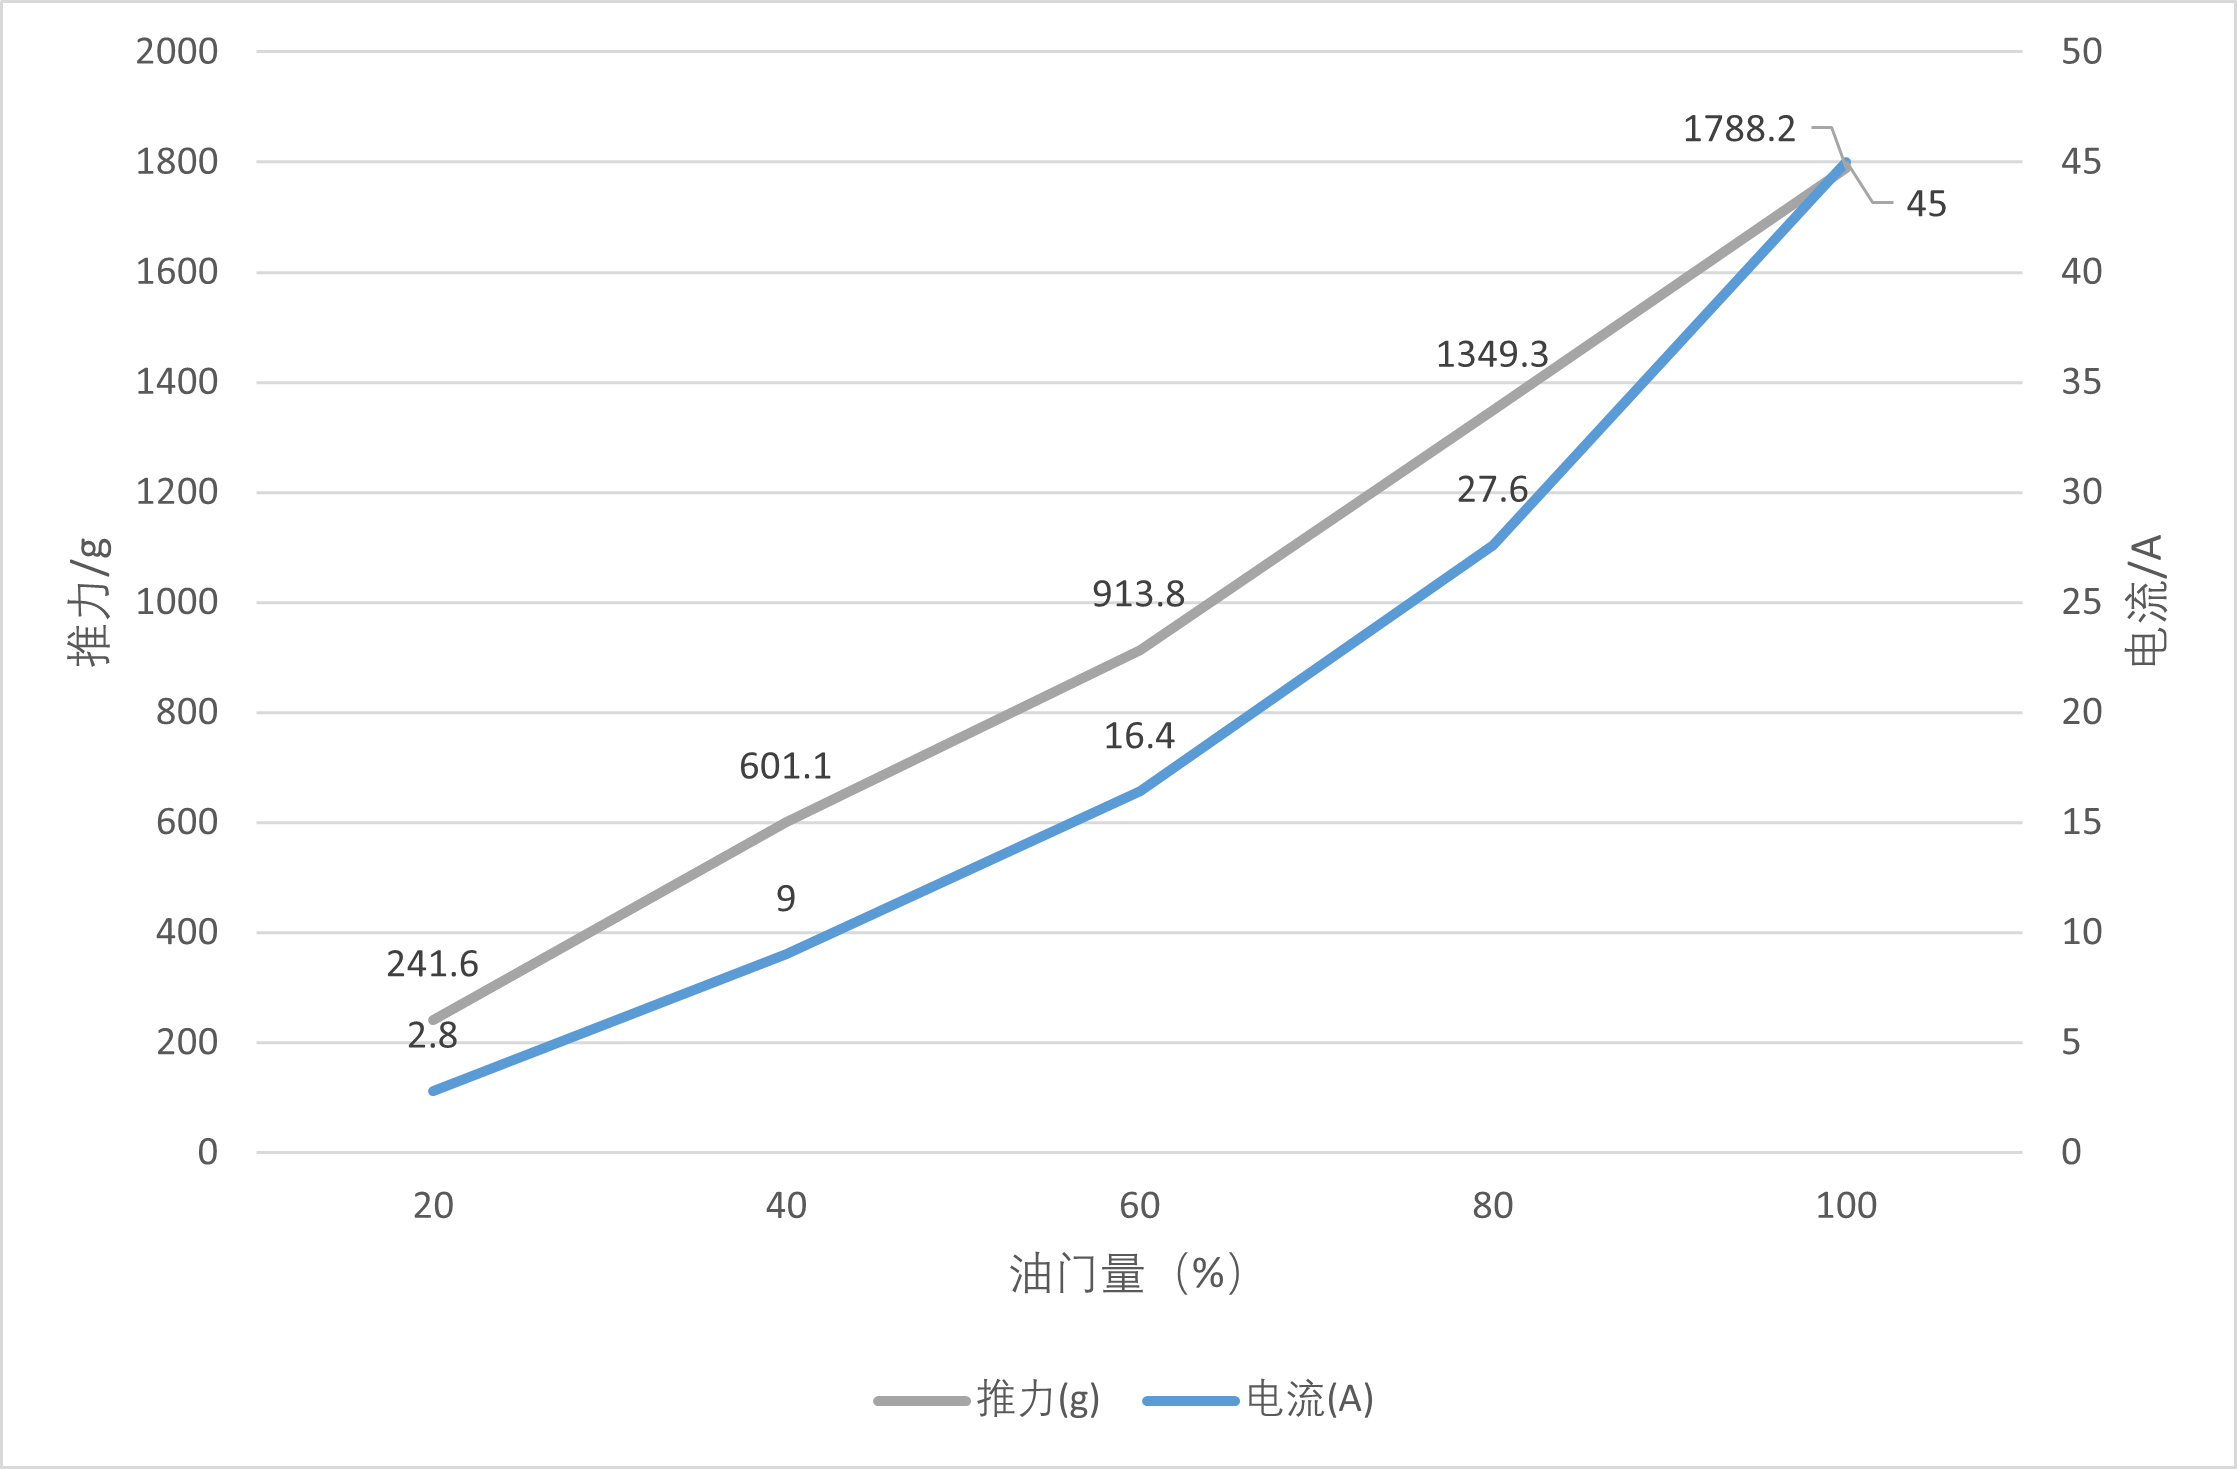
\includegraphics[width=0.7\textwidth]{电机表.png}
  \caption{Tmotor v2207 kv1950电机搭配51477-3螺旋桨 油门量与电流和推力关系图 \cite{Tmotor2023}}
  \label{电机表}
\end{figure}

在几番摸索后,考虑到后续的机载电脑等载荷需要有足够的安装位置,我们选择了holybro品牌的QAV250机架作为平台,以及配套的PM06电源及电调模块,TMOTOR v2207 kv1950电机和pixhawk 6c mini飞控。在装配和接线后,在QGroundControl地面站中对飞控烧写PX4 v1.14版本的固件,并进行传感器校正和遥控器设置。最后,在卫星信号良好的室外进行了遥控器控制下的飞行实验。无人机能够很好地执行遥控器发布的飞行指令,悬停稳定,前进后退自如,飞行效果如图 \ref{室外飞行}。
\begin{figure}[!h]
  \centering
  \begin{subfigure}[c]{0.33\textwidth}
    \centering
    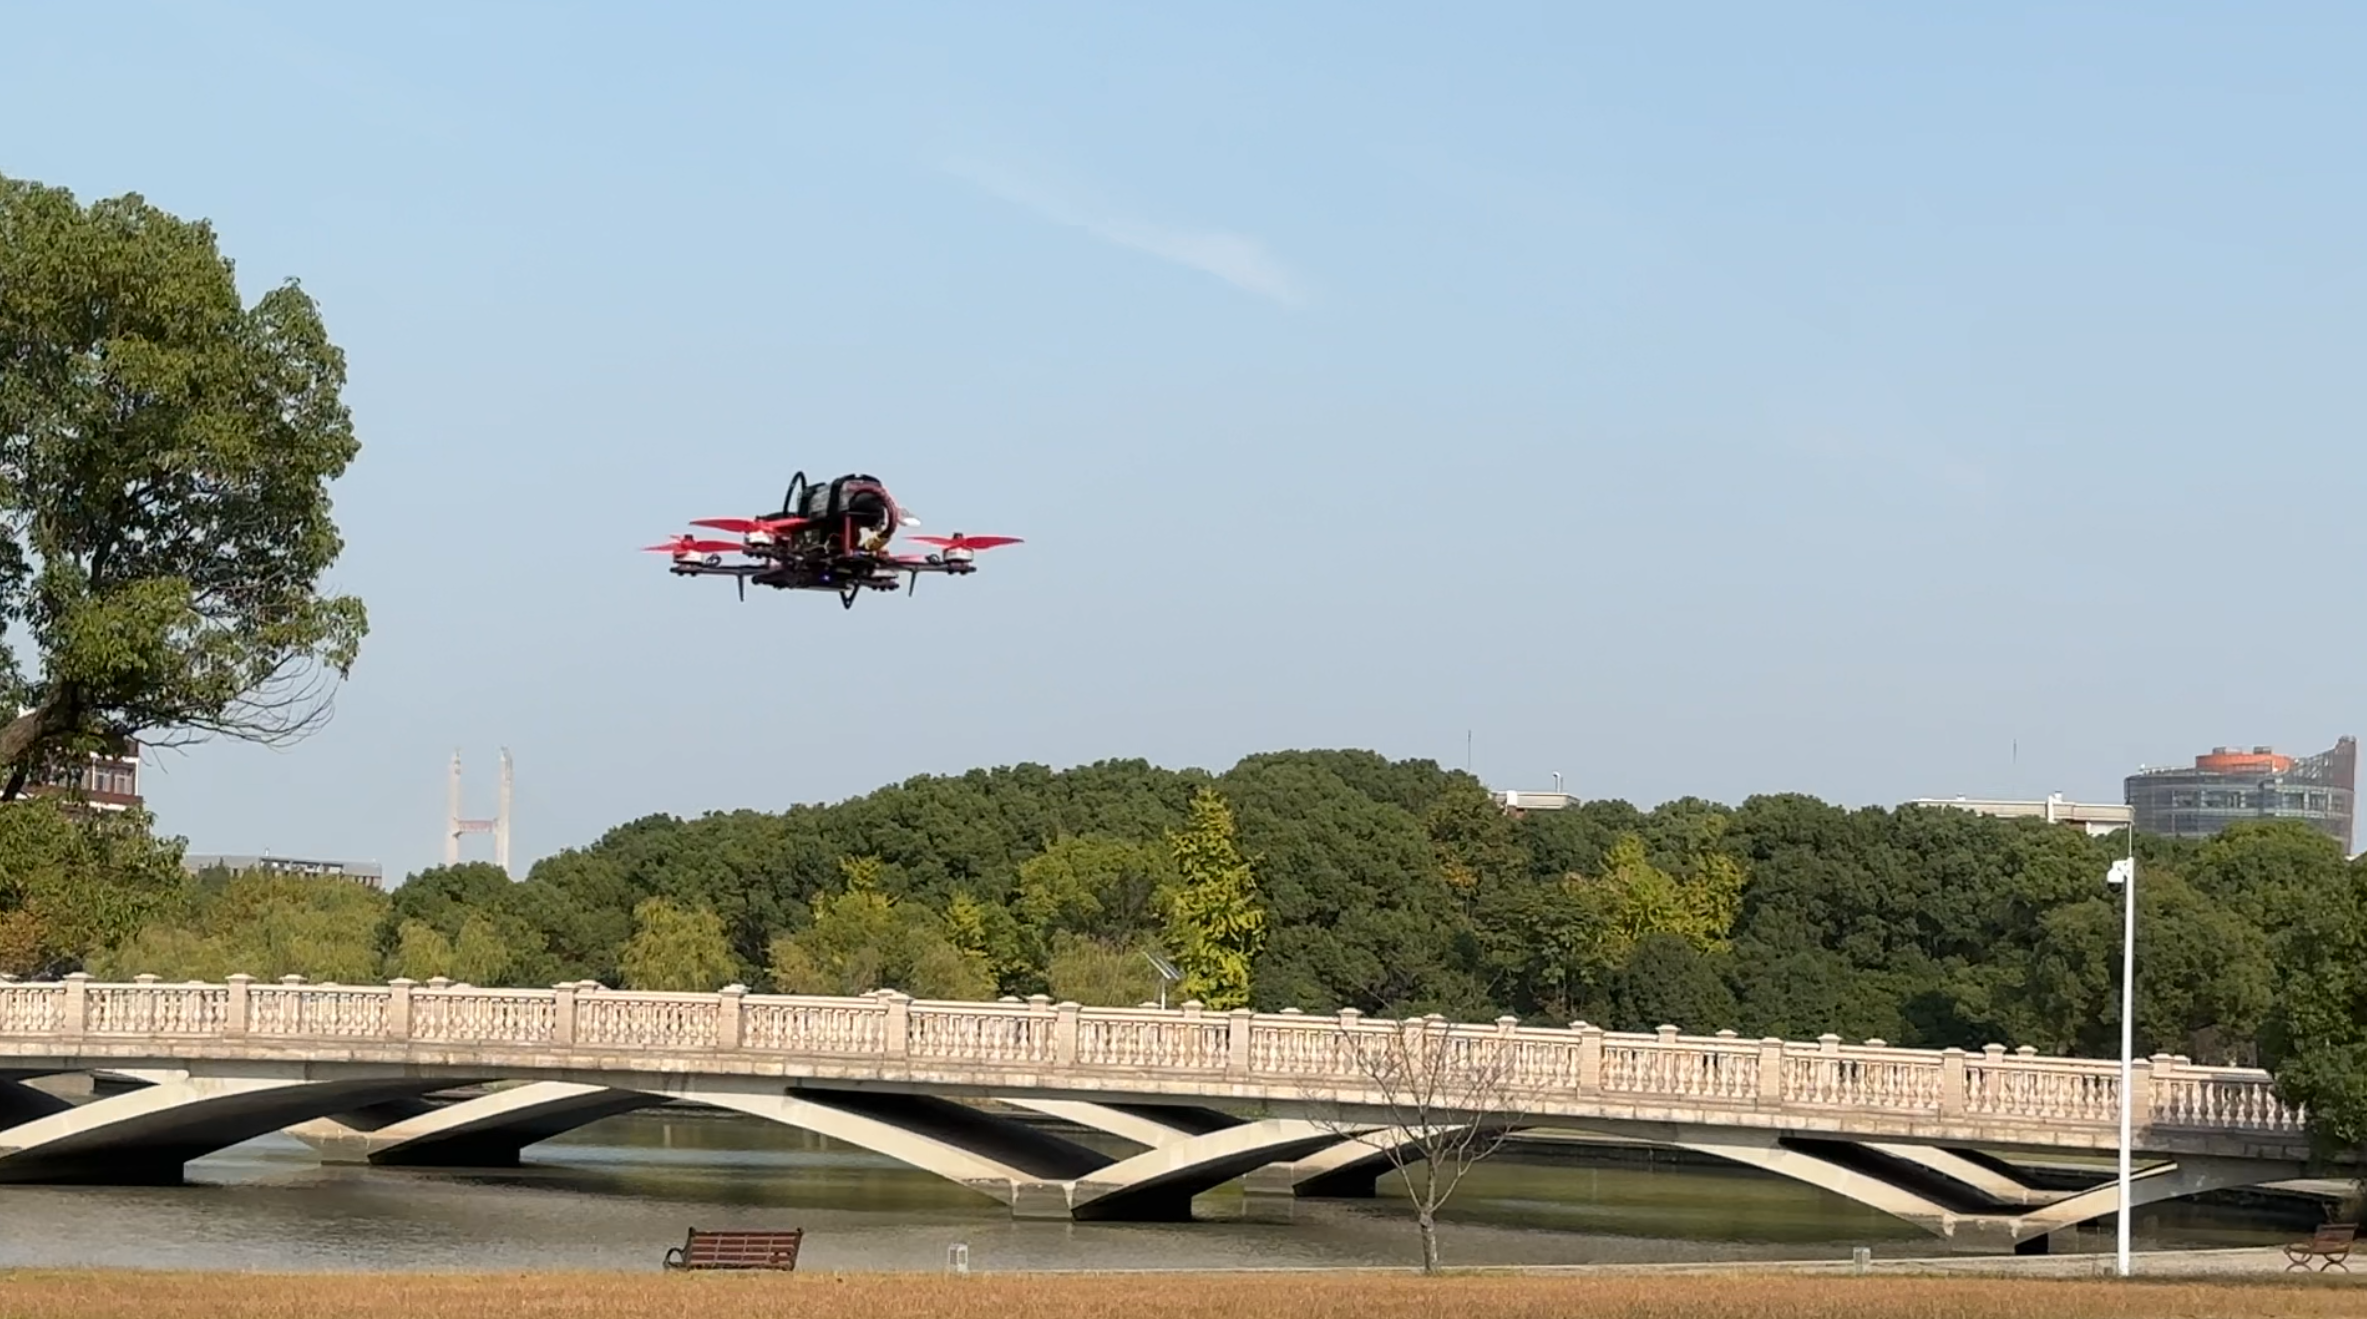
\includegraphics[width=0.95\linewidth]{室外飞行1.png}
  \end{subfigure} \hfill
  \begin{subfigure}[c]{0.33\textwidth}
    \centering
    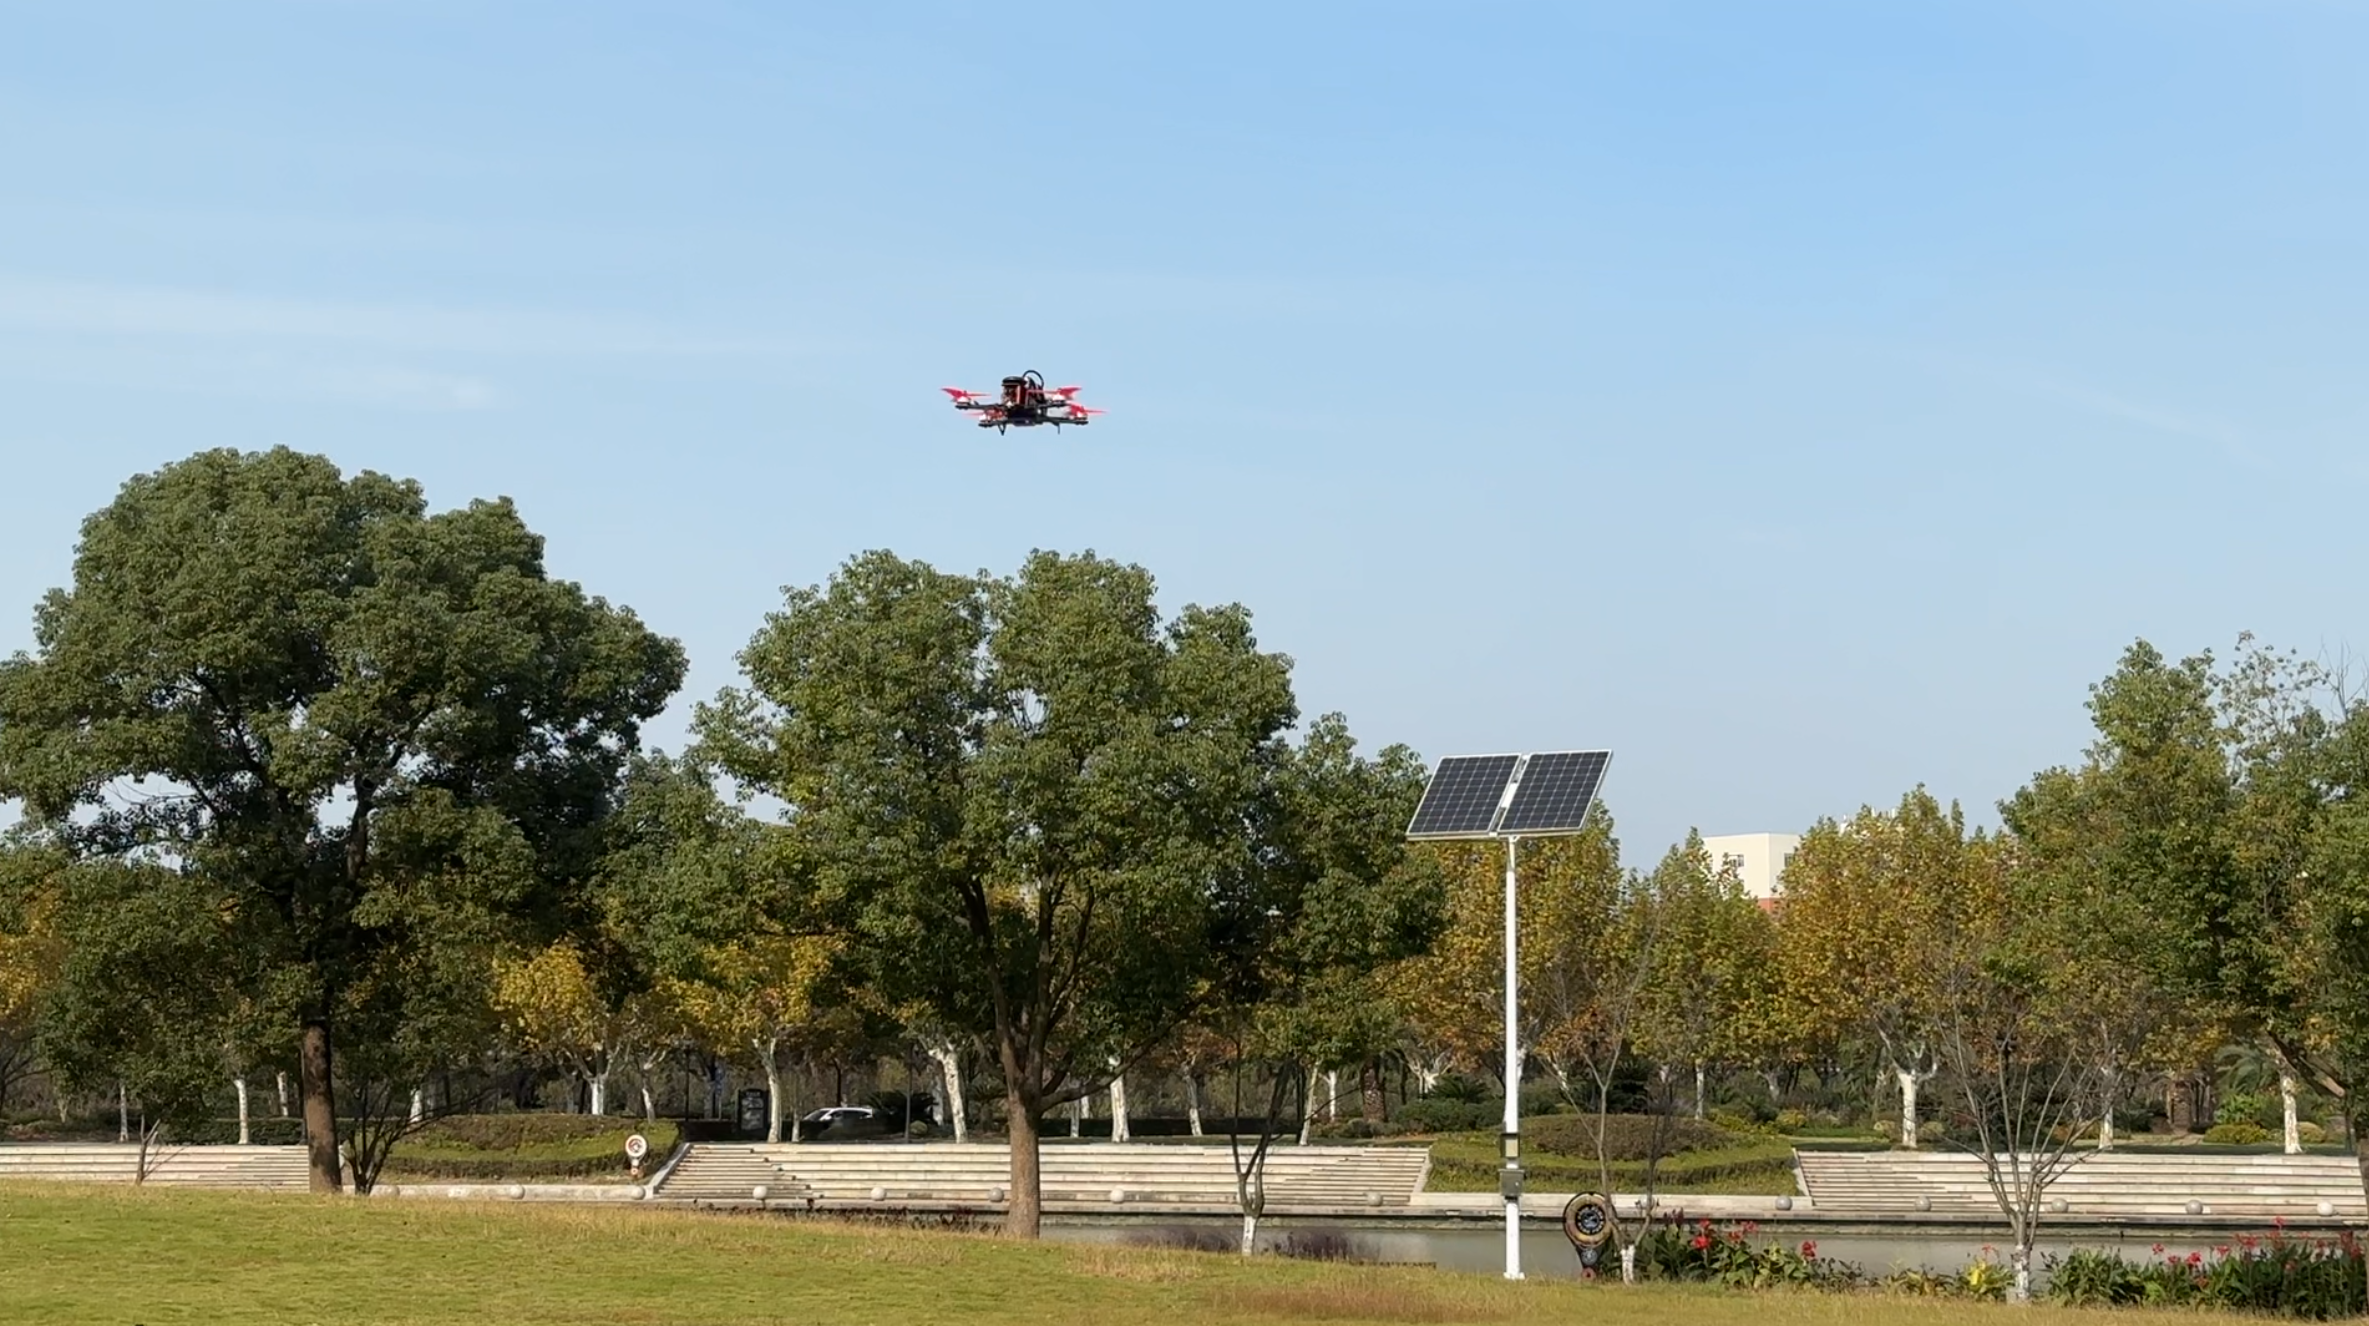
\includegraphics[width=0.95\linewidth]{室外飞行2.png}
  \end{subfigure}\hfill
    \begin{subfigure}[c]{0.33\textwidth}
      \centering
      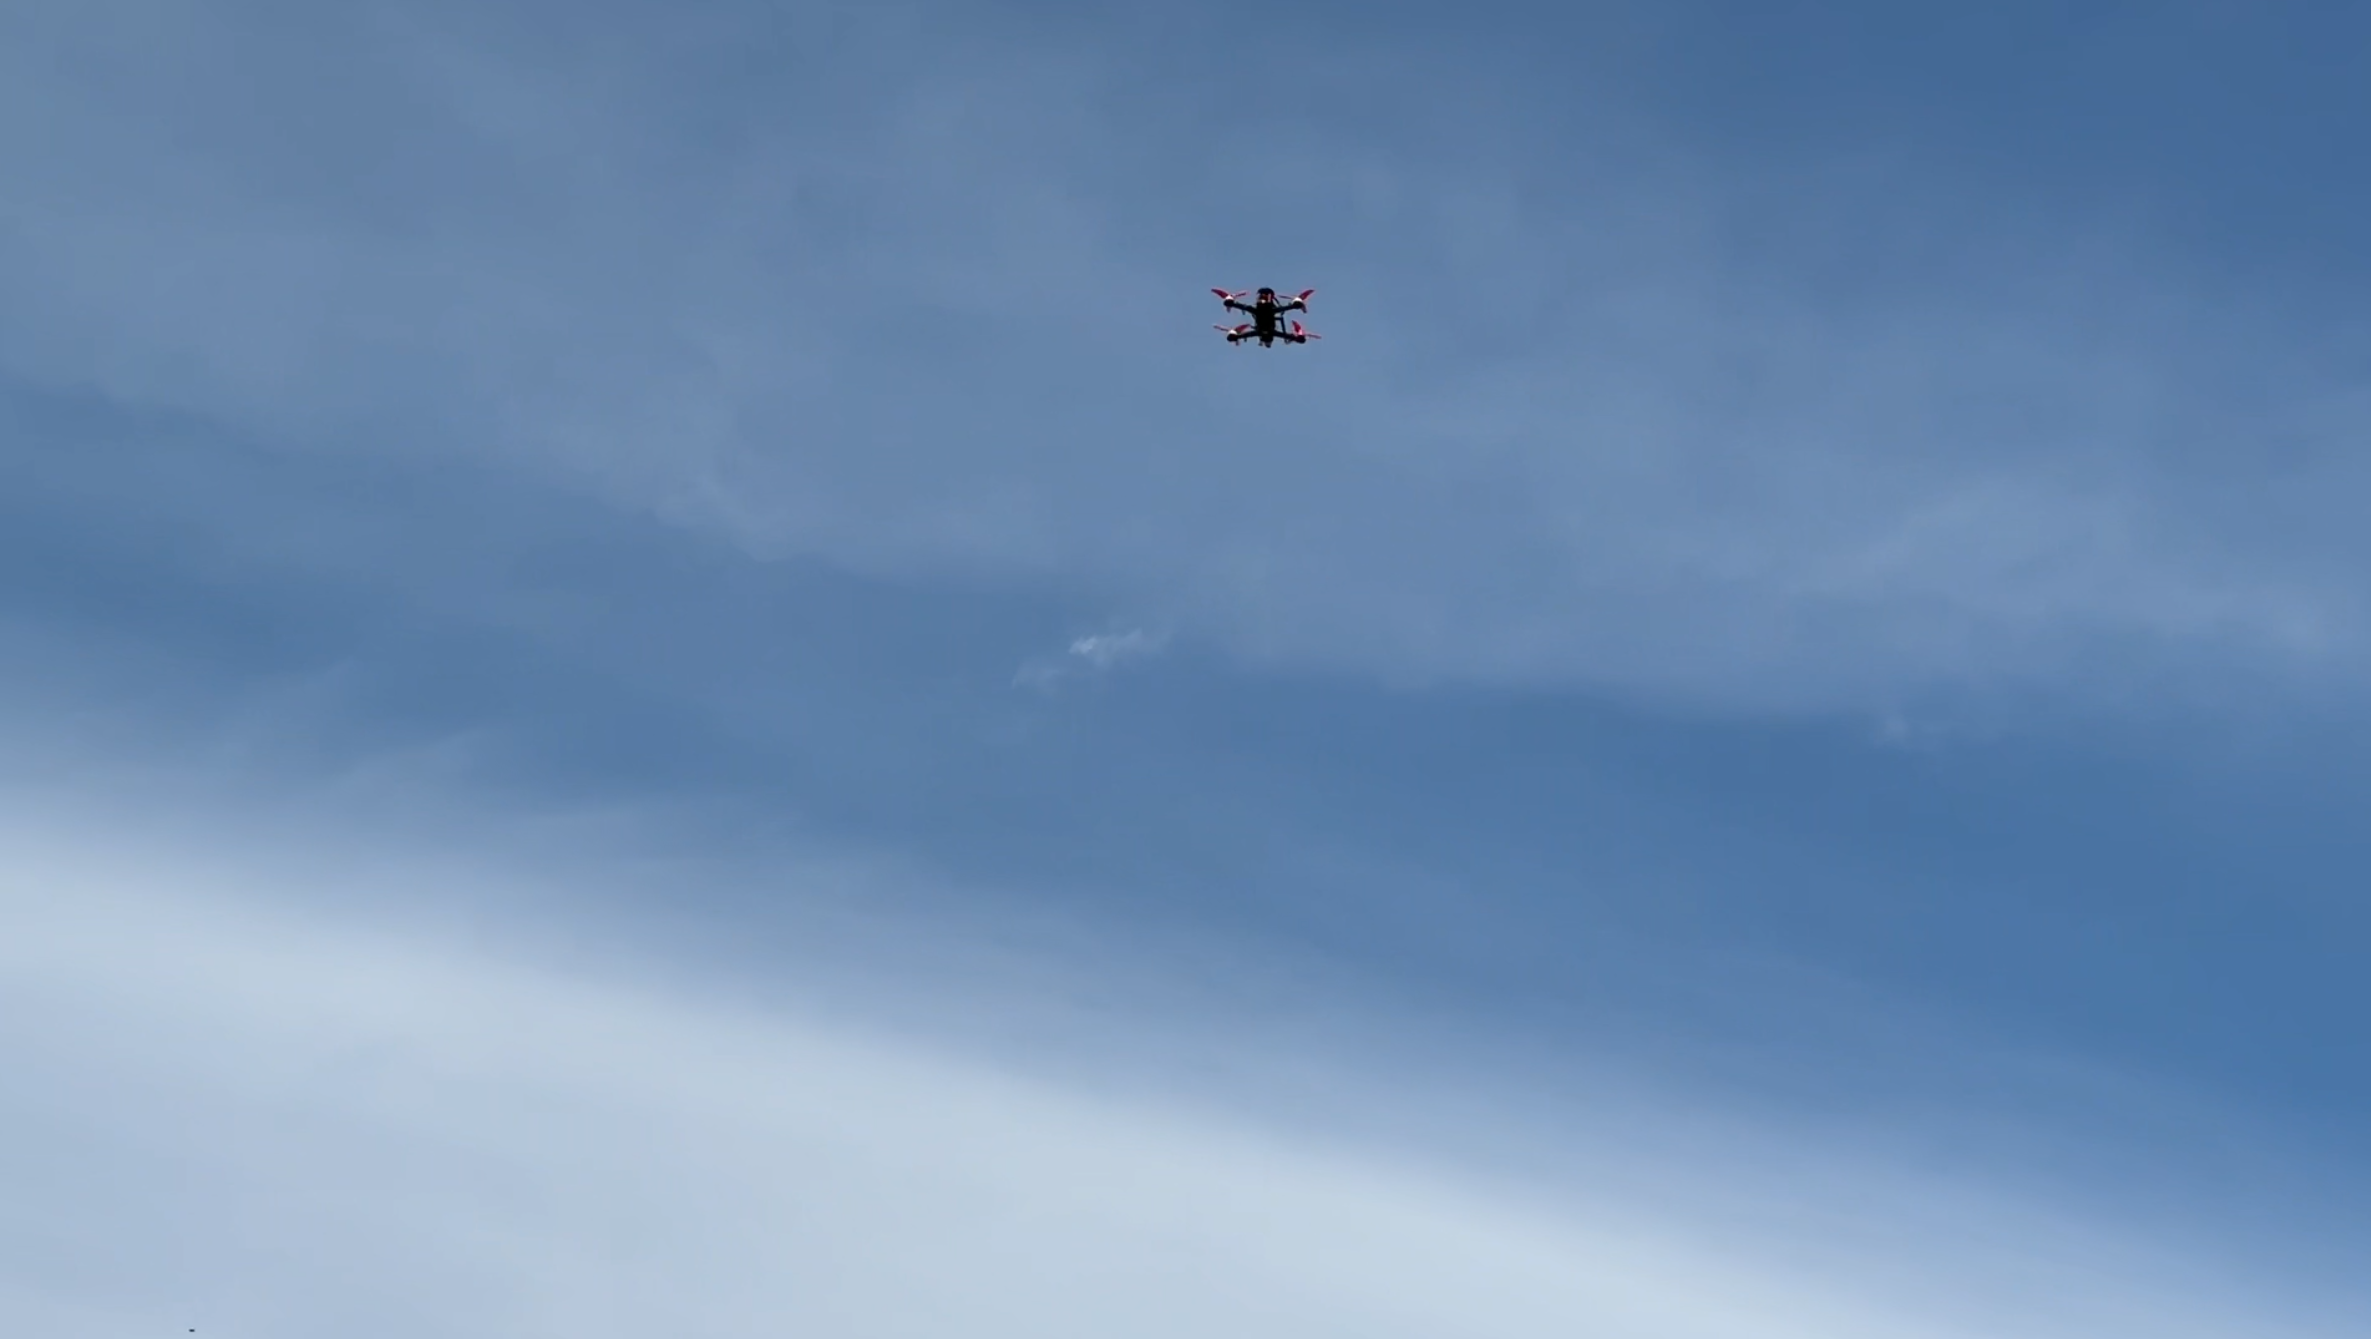
\includegraphics[width=0.95\linewidth]{室外飞行3.png}
  \end{subfigure}
  \caption{位置模式下四旋翼室外飞行画面}
  \label{室外飞行}
  \end{figure}

  \section{基于动捕定位的室内飞行}
室内飞行与室外飞行的主要区别在于位置信息的获得方式。由于室内没有GPS信号,位置信息的获取方式主要有动作捕捉、UWB、自主深度视觉定位和激光雷达等,其中动作捕捉的精度和稳定性最高,并且不用在飞机上增加额外的载荷,所以我们采用了动作捕捉作为本课题的定位方法。
共8台动捕相机吊装在实验场地上方四周,如图\ref{动捕}所示,实验场地的尺寸为$5m \times 4.6m \times 2.6m$。在当前配置下,可以达到亚毫米的定位精度和400hz的采样频率\cite{qingtong}。
\begin{figure}[!h]
  \centering
  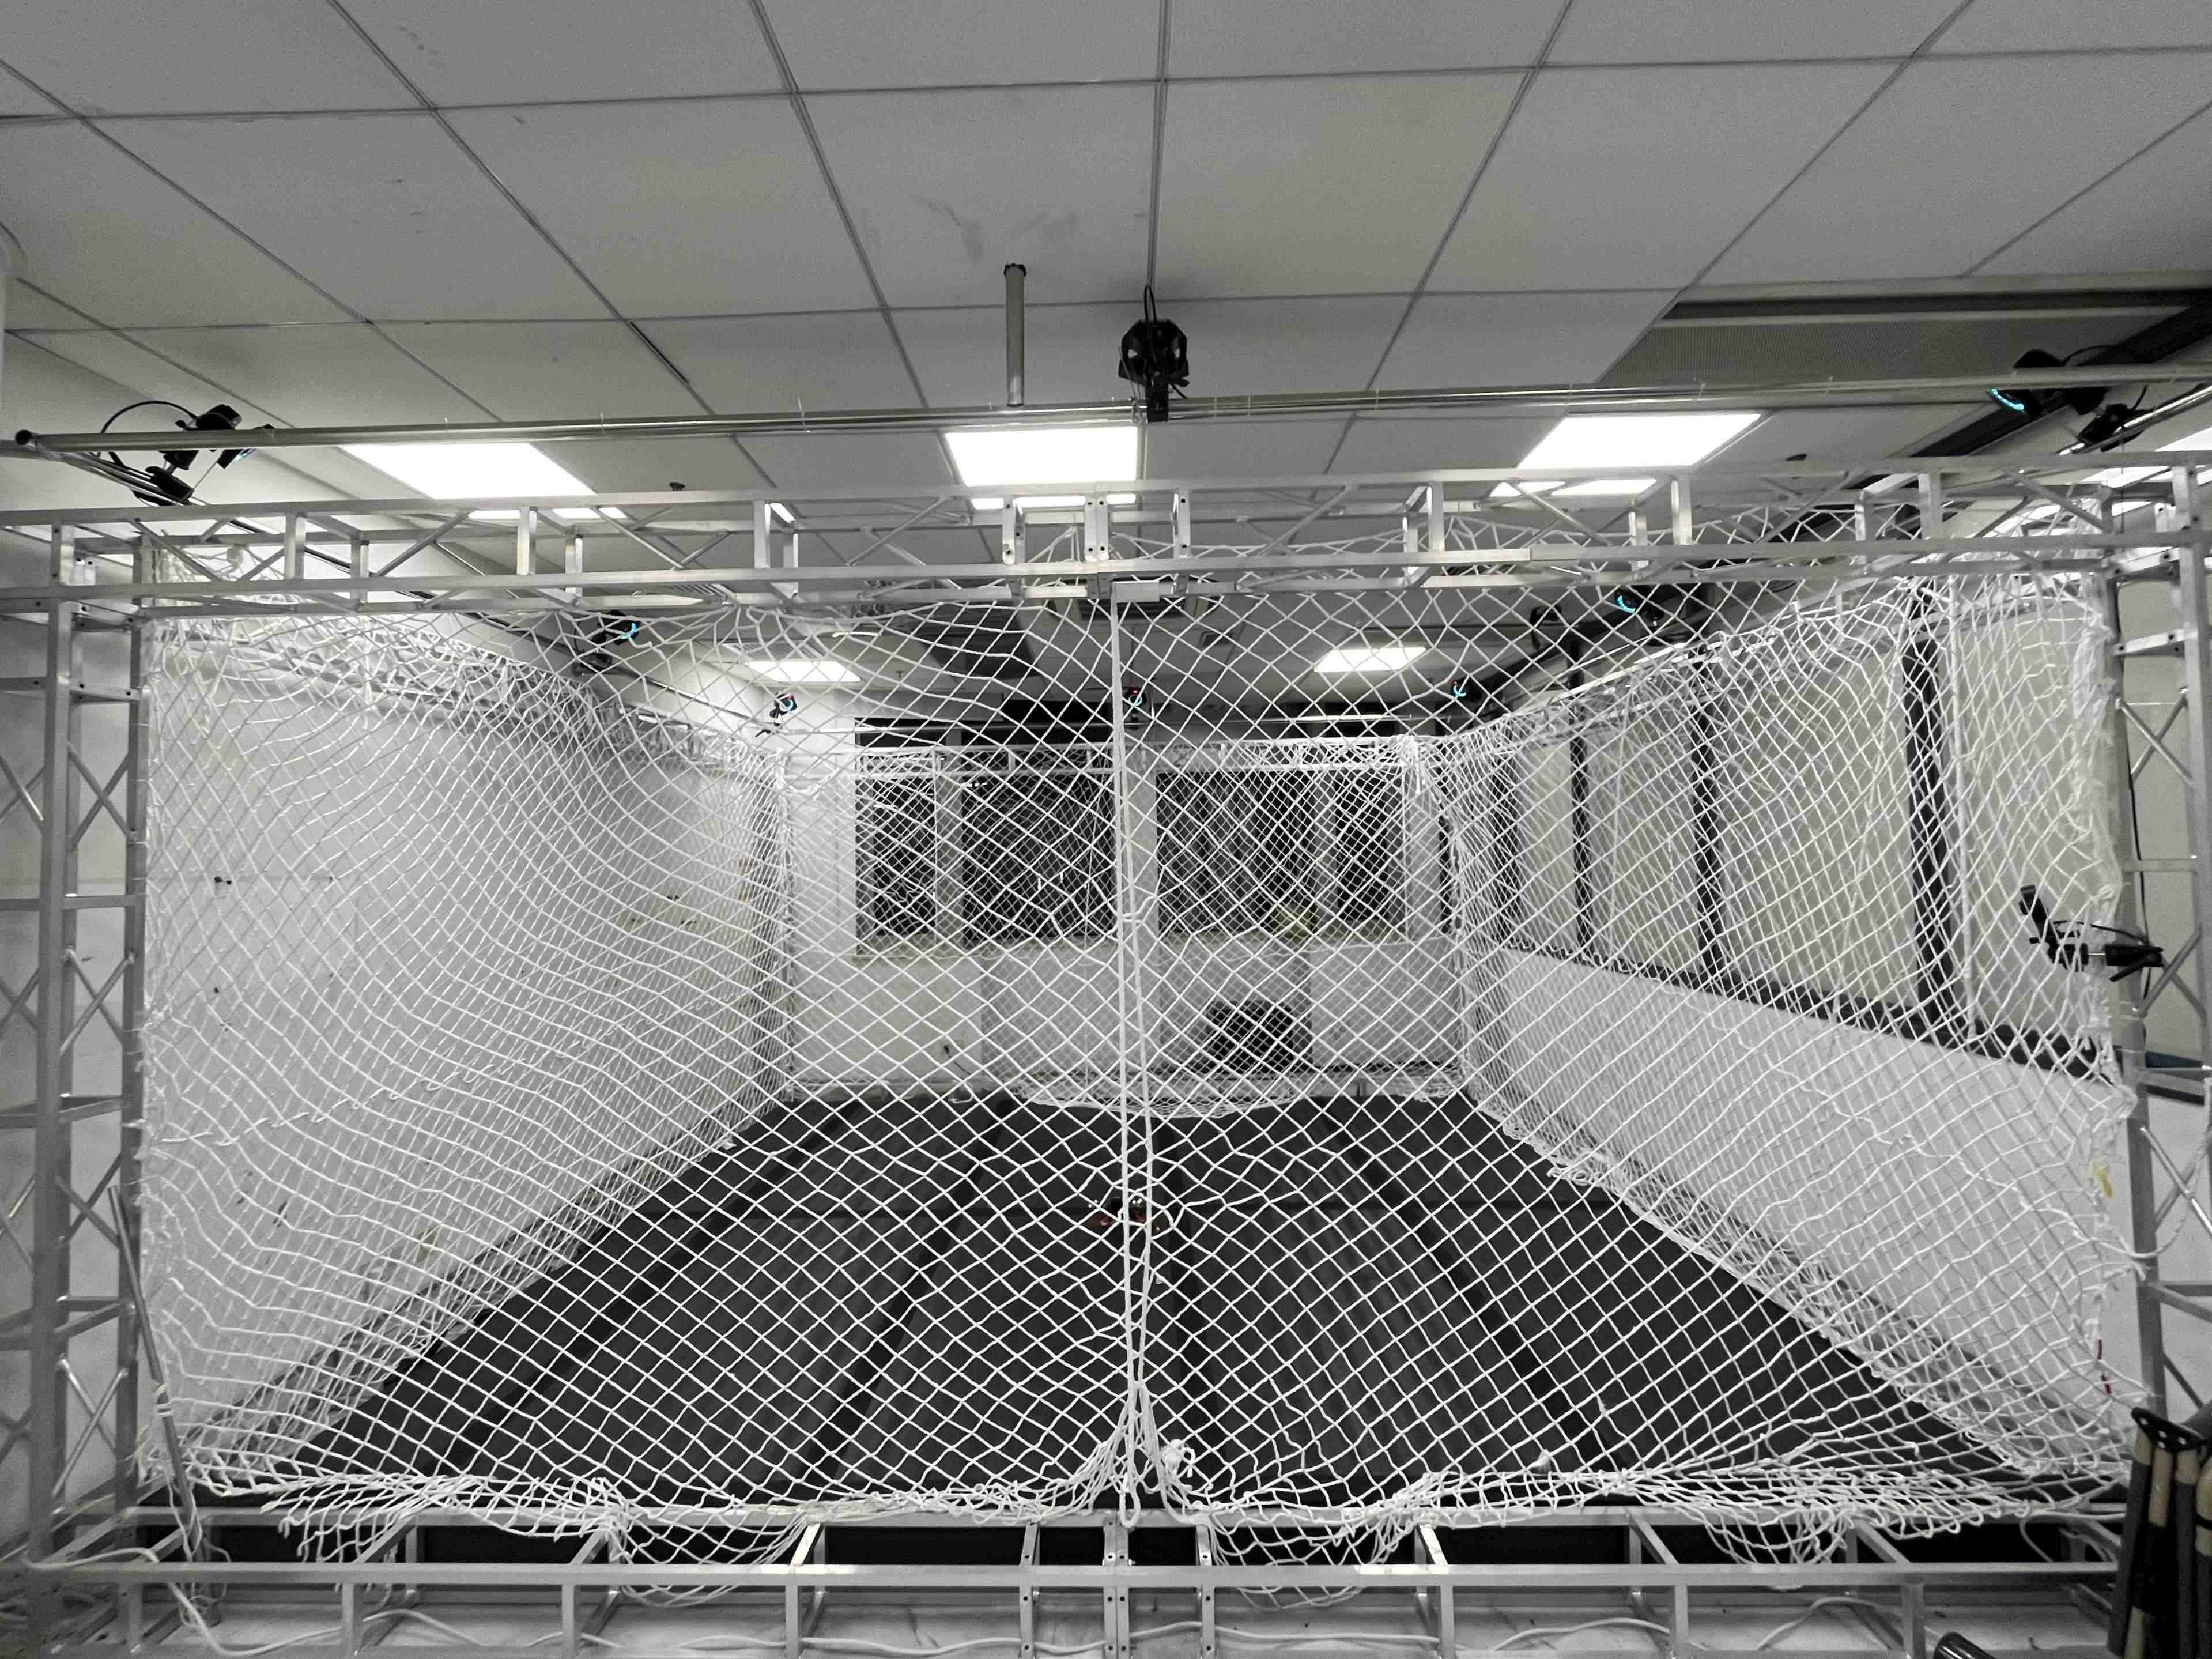
\includegraphics[width=0.6\textwidth]{动捕.jpg}
  \caption{动捕系统以及无人机防撞绳网}
  \label{动捕}
\end{figure}
动捕系统使用红外相机向目标发射红外光,使目标上固连的多个反光小球(marker)反射红外光,就能使相机捕捉到,效果如图\ref{反光小球}。


\begin{figure}[h]
  \centering
  \begin{subfigure}[c]{0.4\textwidth}
    \centering
    \includegraphics[width=0.95\linewidth]{飞机反光球.jpg}
    \caption{marker安装方式}
  \end{subfigure}\hfill
    \begin{subfigure}[c]{0.55\textwidth}
      \centering
      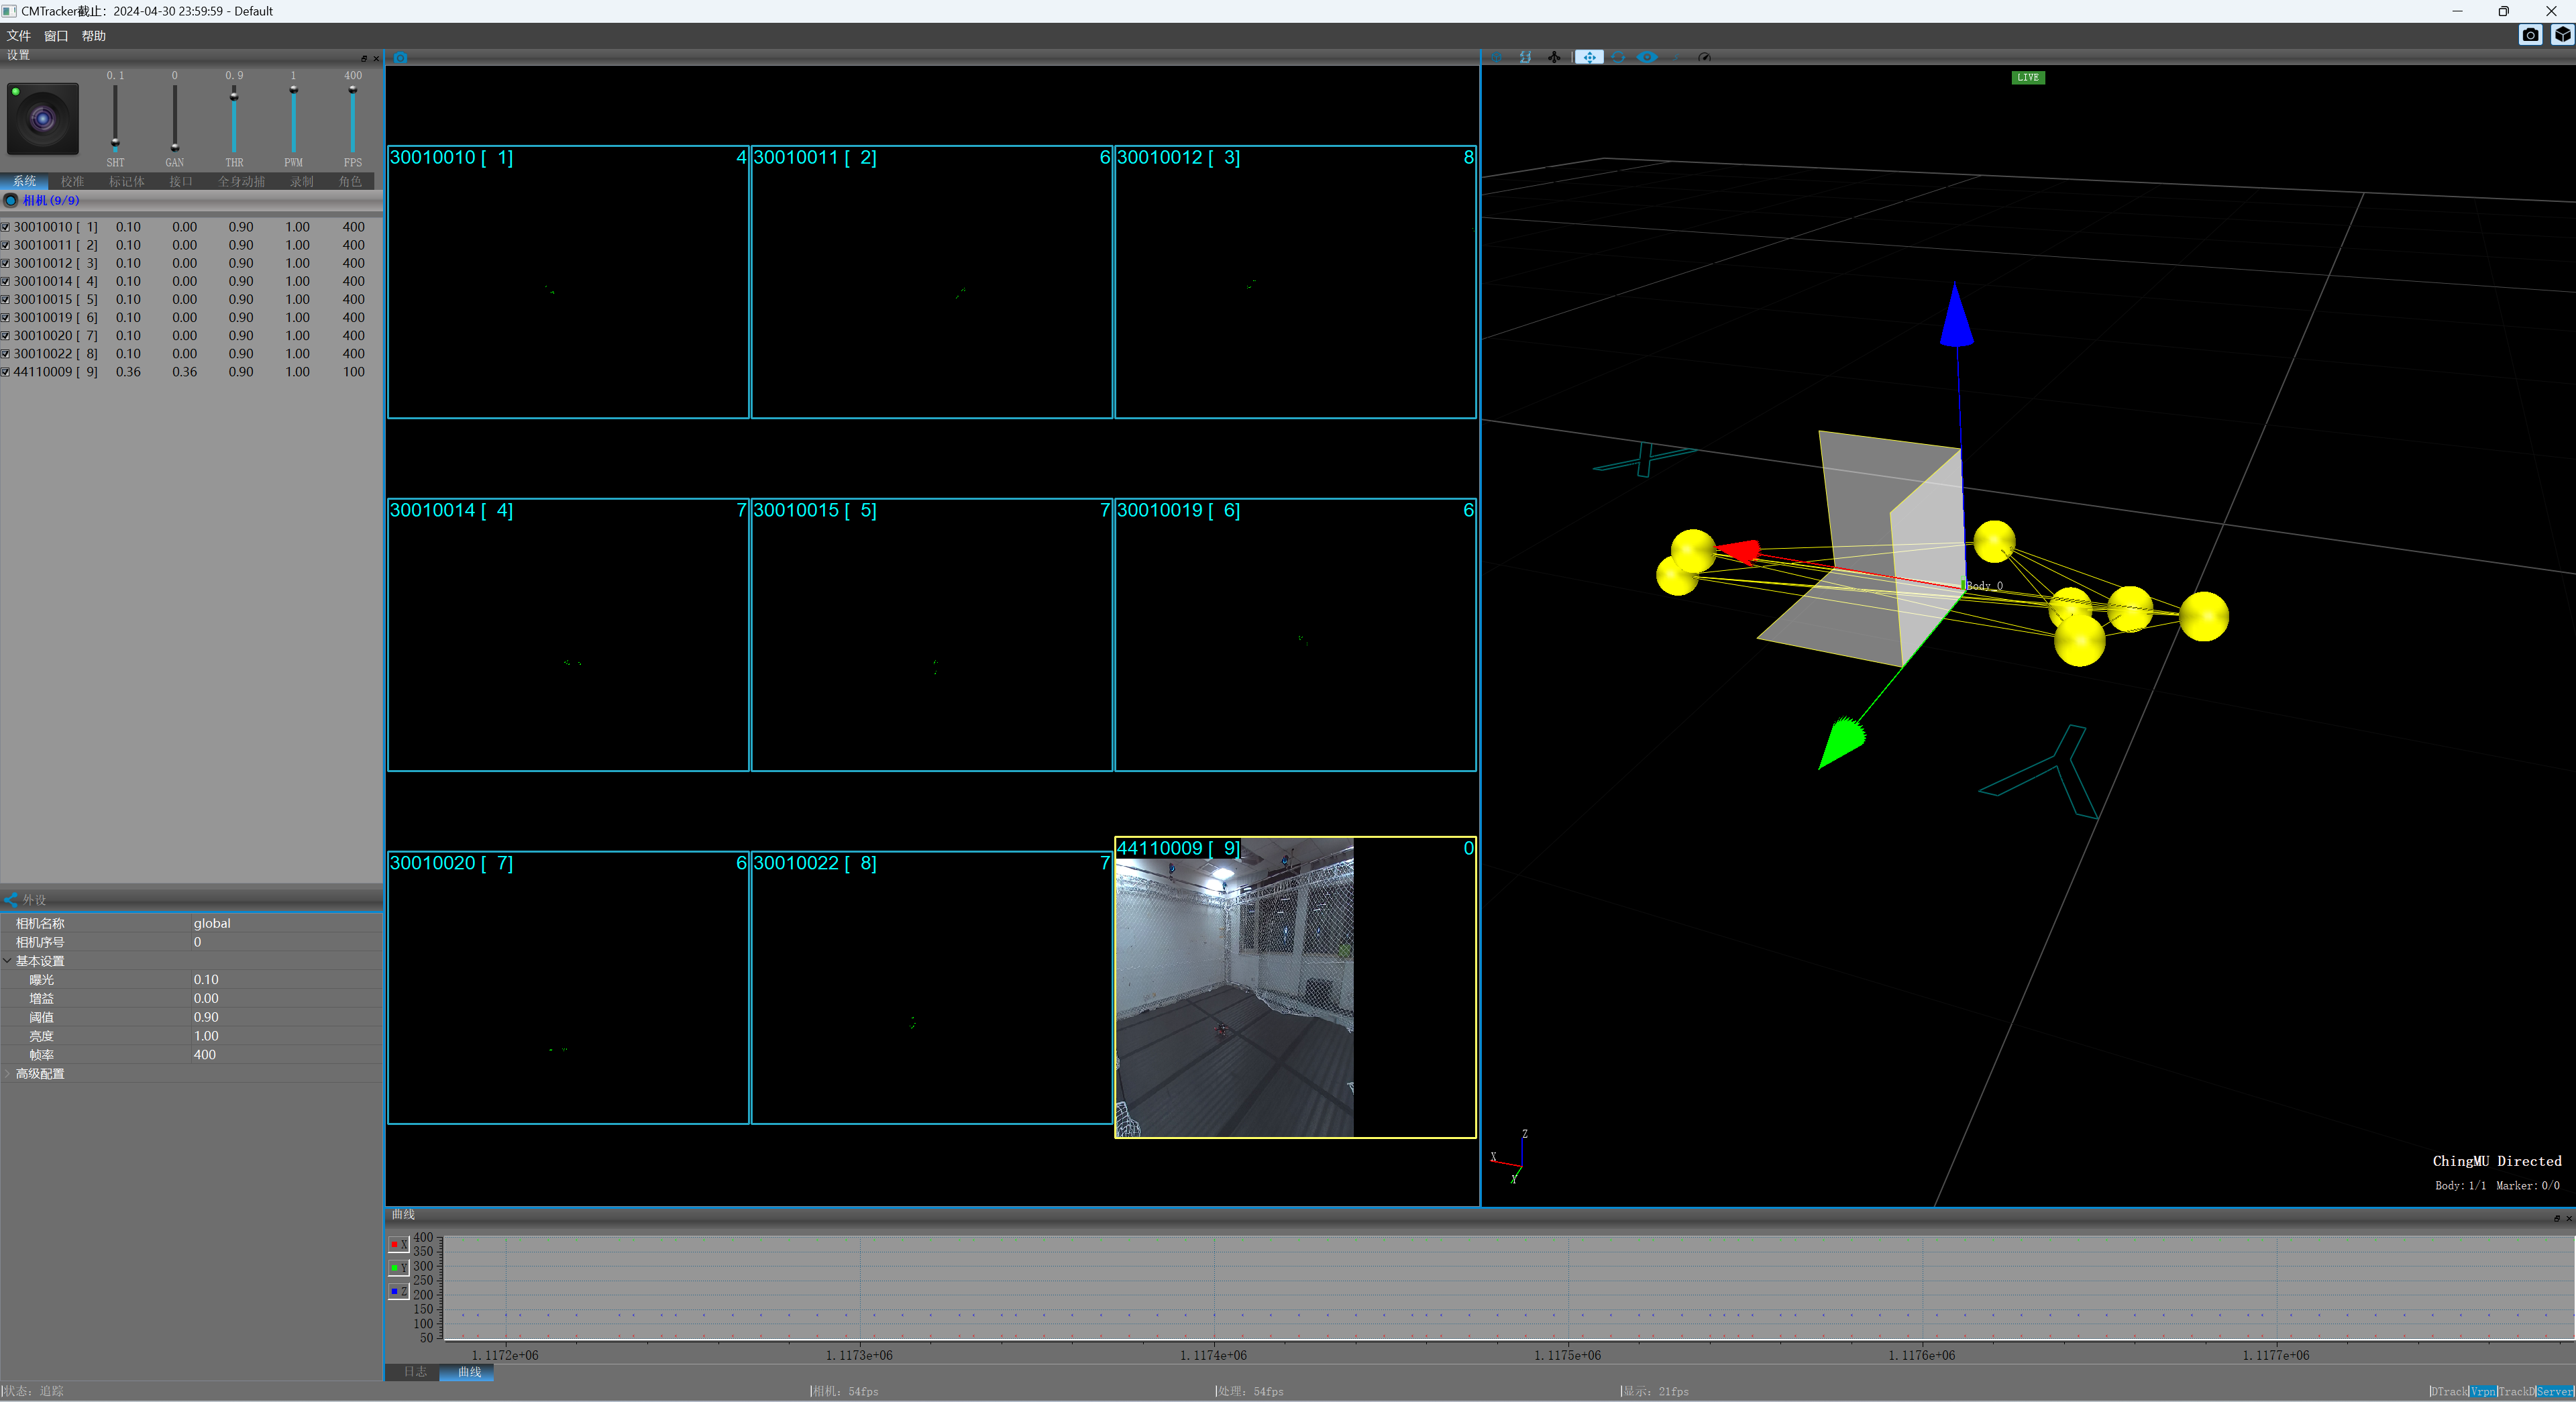
\includegraphics[width=0.95\linewidth]{动捕效果2.png}
      \caption{动捕系统界面}
  \end{subfigure}
  \caption{动作捕捉系统定位marker}
  \label{反光小球}
  \end{figure}


由于相机通过扫场校准已知自身位置,多台相机的二维信息融合在一起就可以解算出目标的位置和姿态。
相机在拍到反光小球后首先在内部做一次图像处理,提取反光点位置,然后通过网线传到动捕服务器上。所有的相机和东部服务器都通过网线连在一台交换机上,形成一个局域网。动捕服务器在汇总了所有信息后解算出目标刚体的位置和姿态,然后以固定的数据报协议在其所在的所有局域网内广播。动捕服务器在用网线连接交换机之外,还和机载电脑连接同一个wifi,也就是说动捕服务器同时处在两个局域网中,而机载电脑也可以通过wifi这个局域网收到位姿广播。

在ros1的架构下,飞控和电脑需要存在有线连接才能通过运行mavros包下的px4.launch,经/dev/ttyACM0端口,将飞控虚拟化为一个ros节点。同时运行vrpn-client-ros包内的sample.launch,接受局域网内的位姿广播。最后运行topic-tools relay命令,将位姿信息转发到mavros节点下的vision-pose/pose话题。运行rqt-graph命令得到消息拓扑图\ref{rqt}。

\begin{figure}[!h]
  \centering
  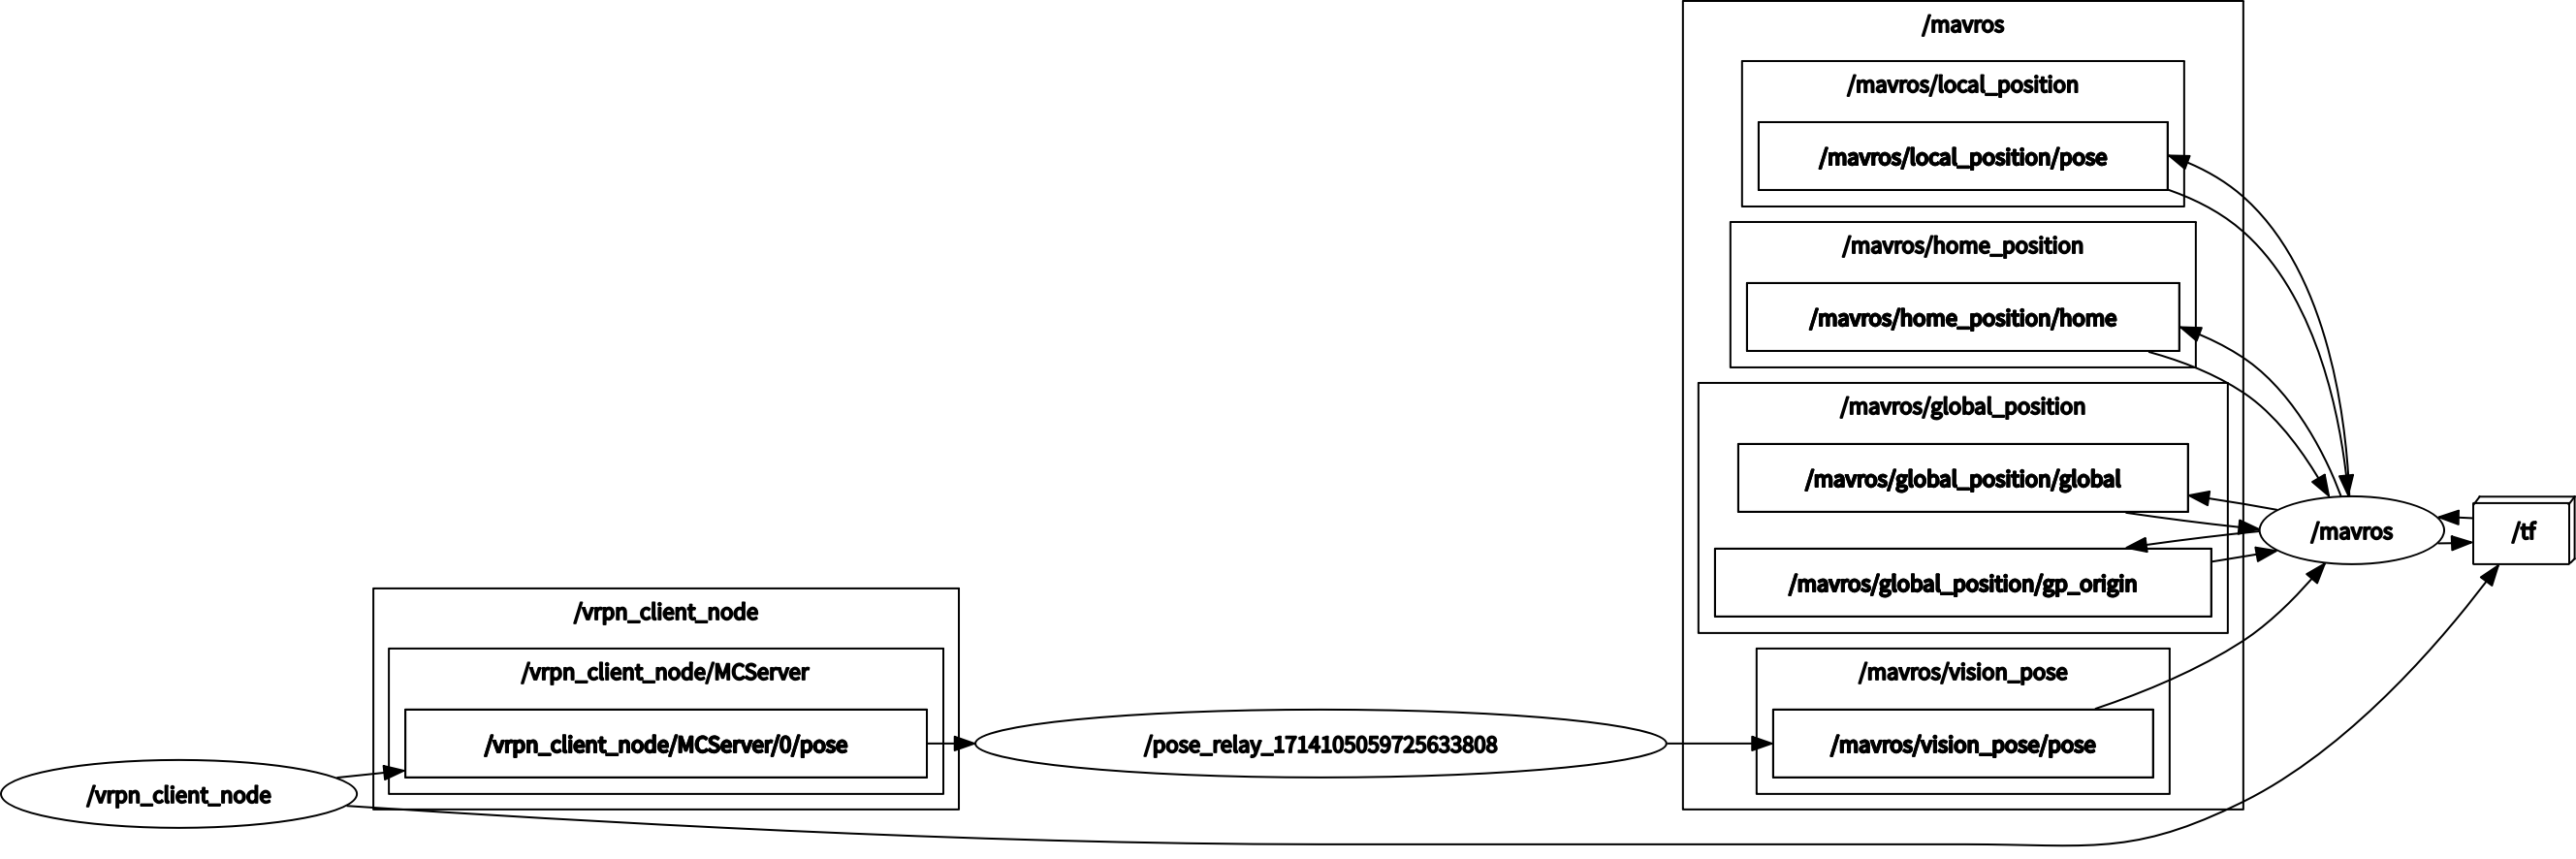
\includegraphics[width=0.9\textwidth]{rqt.png}
  \caption{消息拓扑图}
  \label{rqt}
\end{figure}

以上的这三部分命令可以写到一个bash文件中一键运行,如图 \ref{一键},其中运行px4.launch的参数有gcs-url,这是地面站的ip地址和端口号。
\begin{figure}[!h]
  \centering
  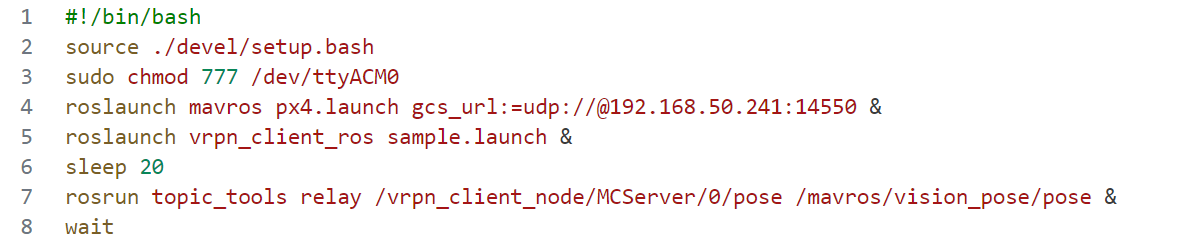
\includegraphics[width=0.8\textwidth]{bash.png}
  \caption{一键启动命令}
  \label{一键}
\end{figure}
mavros会通过wifi与地面站连接,地面站的QGroundControl(QGC)中就能方便地看到无人机目前的状态信息(当然也能通过rviz或rostopic等工具看到),如图 \ref{qgc},也能够发布起飞等指令。
\begin{figure}[!h]
  \centering
  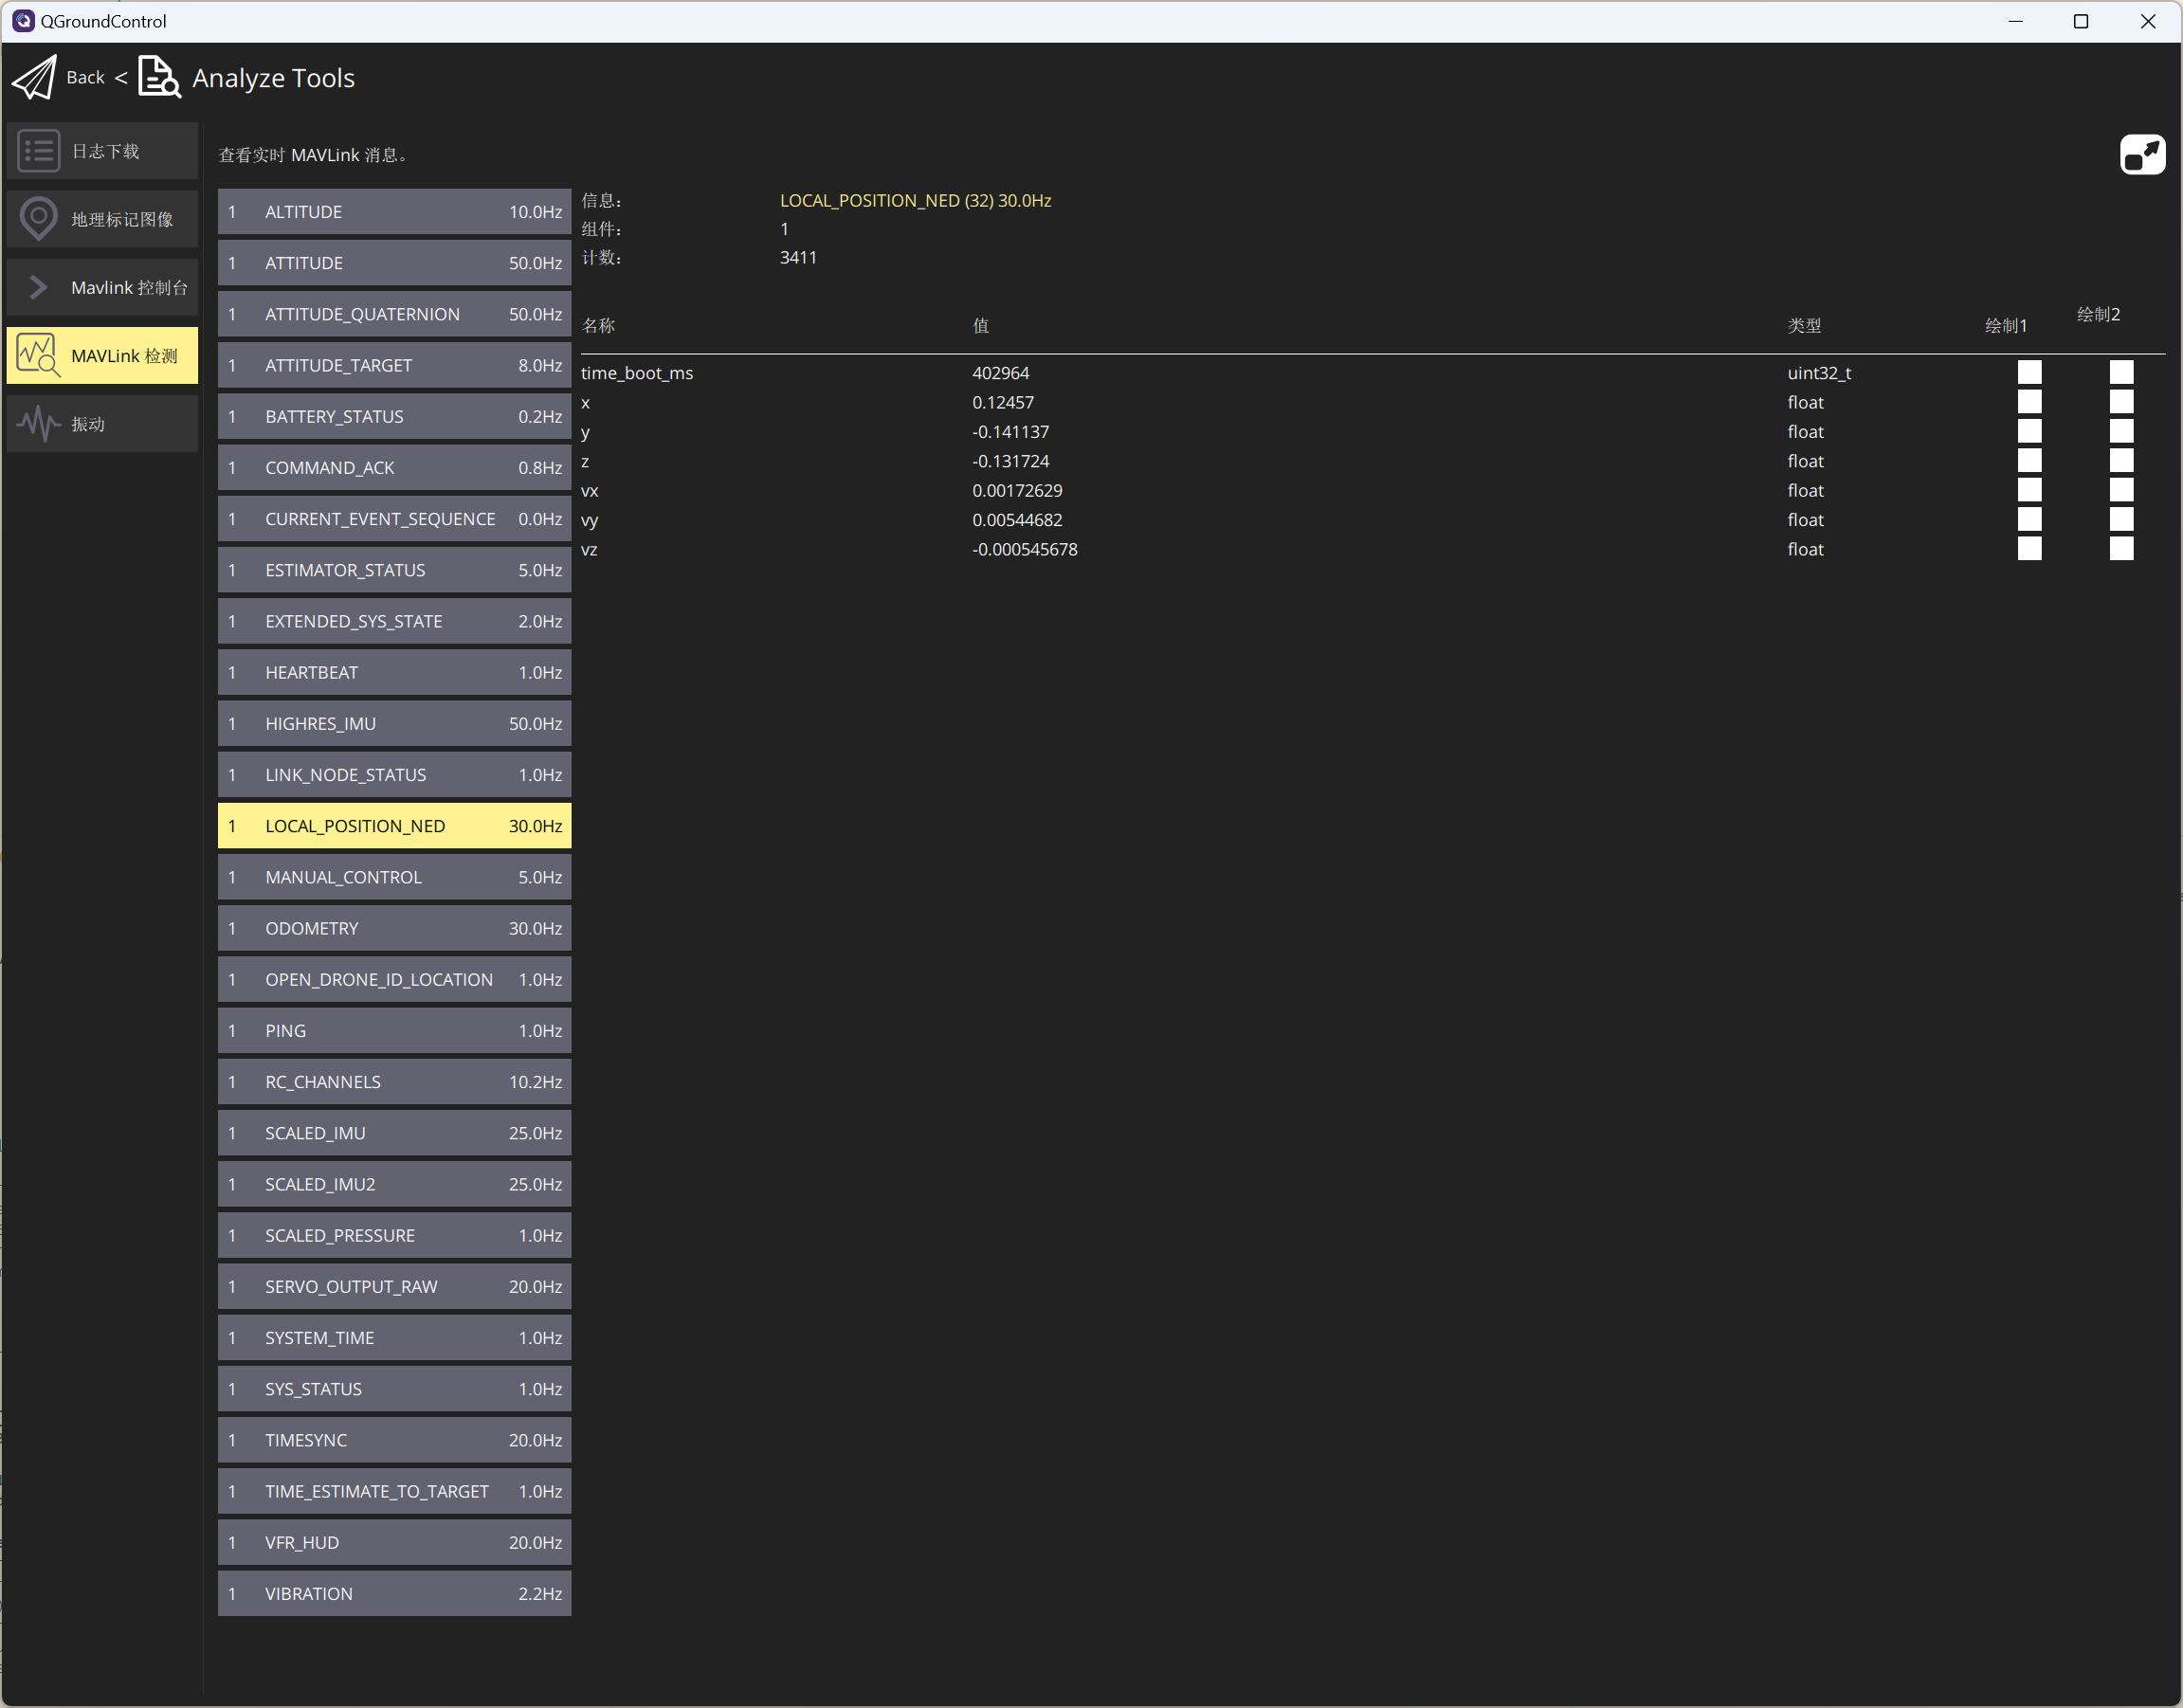
\includegraphics[width=0.5\textwidth]{qgc.png}
  \caption{无人机向QGroundControl传回的信息}
  \label{qgc}
\end{figure}
\newpage
动捕和飞控内部会各自生成两套坐标系,它们的对齐需要着重考虑。如图 \ref{动捕效果},动捕中无论是全局的坐标还是机身坐标,z轴都是朝上,而如1.2.1节中所说,PX4以及本课题定义的坐标系都是z轴朝下。但由PX4向ros提供的mavros包里,已经考虑了这一点,因为市面上的动捕系统大多都使用z轴朝上的配置。只需要注意飞控上电时的机头指向与动捕中的x轴对齐,z轴朝上,就能对齐两套坐标系\cite{px4},而不用关注无人机上电时的位置。PX4内部进行数据融合是会以动捕信息的位置初始值为准,也就是只要方向正确,在场地内的任何地方上电都会按照动捕系统的坐标系配置。
\begin{figure}[!h]
  \centering
  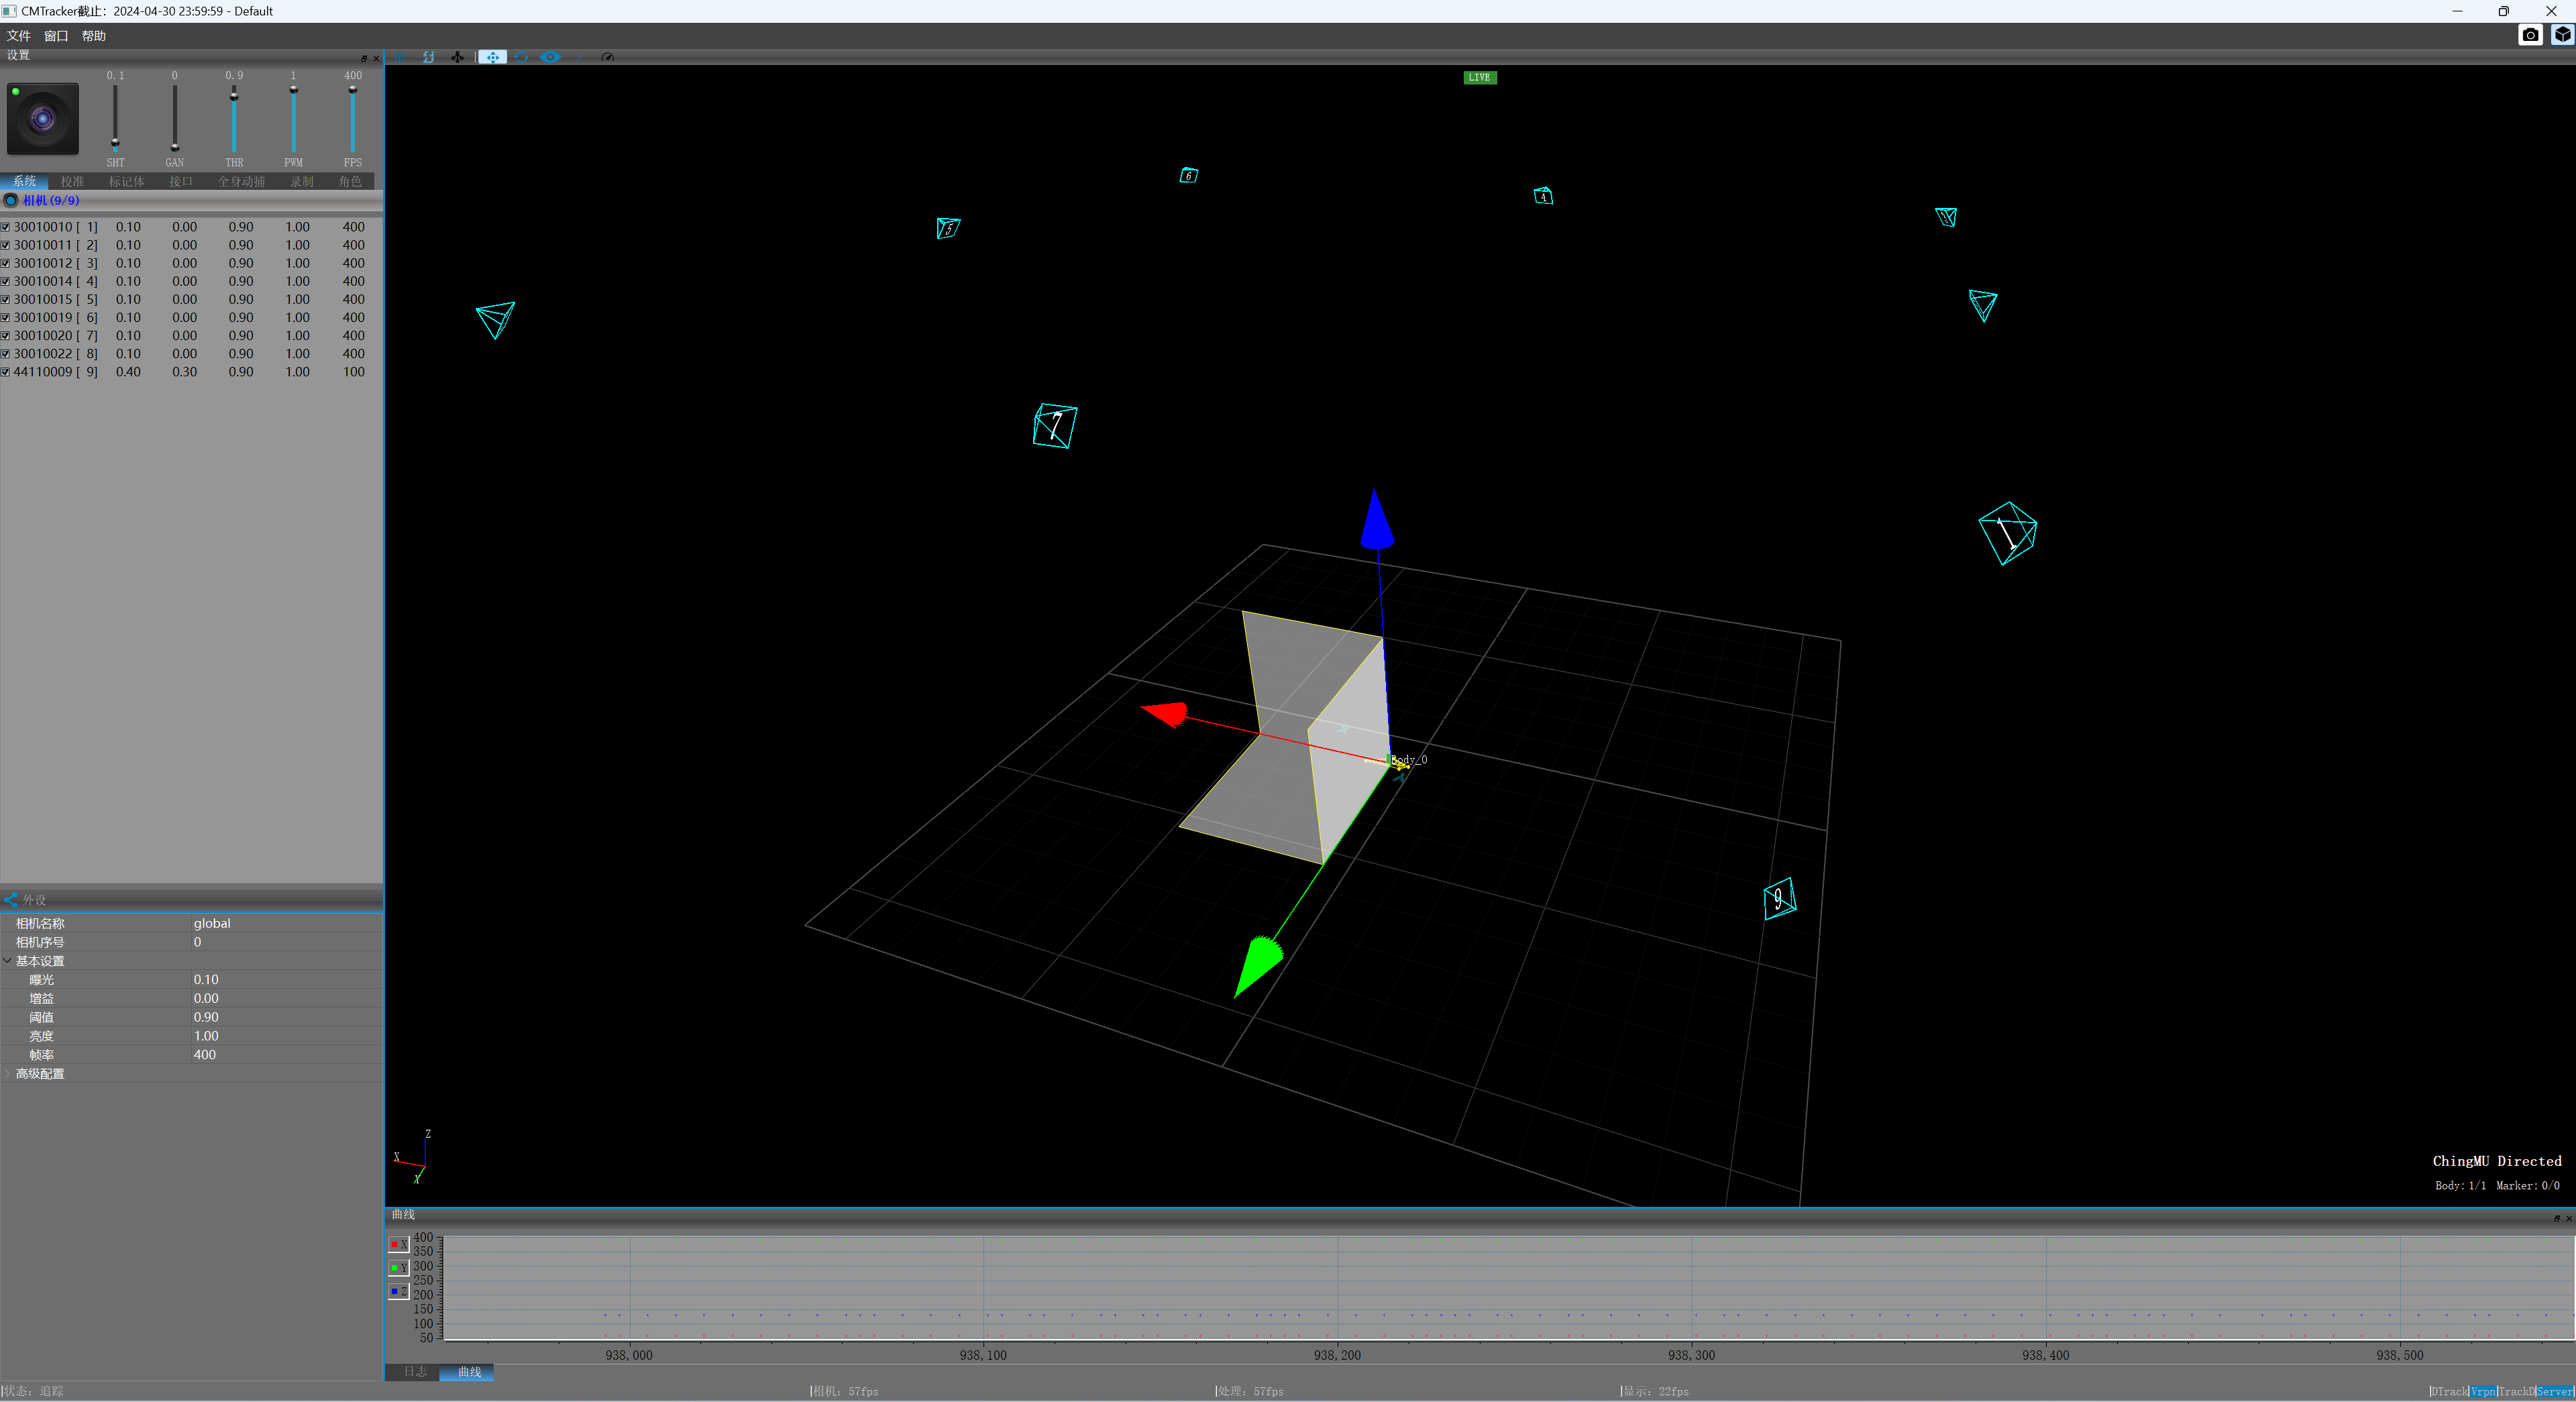
\includegraphics[width=0.6\textwidth]{动捕效果1.png}
  \caption{动捕坐标系设定}
  \label{动捕效果}
\end{figure}

在QGC中查看传回来的位姿信息,多方向移动无人机查看位置变化是否如预期,旋转无人机查看姿态变化是否如预期。需要注意的是QGC中PX4的LOCAL-POSITION-NED、ATTITUDE-QUATERNION、ATTITUDE等话题的坐标系与动捕的坐标系并不相同,如PX4官方文档\cite{px4}中示意图所示 \ref{mocpx4}。z轴由朝上改为朝下,x轴与y轴互换,机身坐标系亦是如此(初始时机身坐标系与世界坐标系重合),这也就意味着上电时动捕坐标系下姿态四元数为幺元,而在PX4的坐标系中绕z轴有$90  ^{\circ}$ 的旋转。
\begin{figure}[!h]
  \centering
  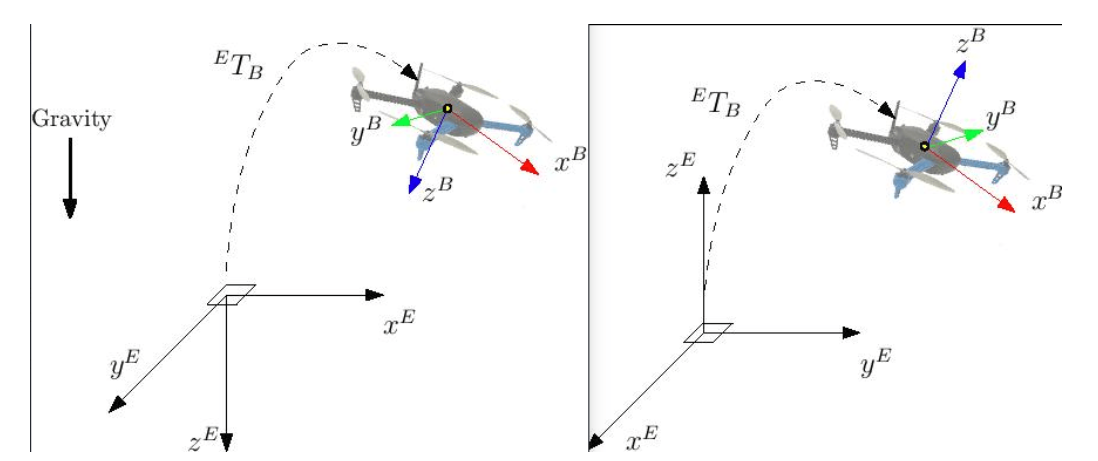
\includegraphics[width=0.7\textwidth]{mocpx4坐标.png}
  \caption{左侧为PX4内坐标系 右侧为动捕系统坐标系}
  \label{mocpx4}
\end{figure}

在上述检查确认无误后,可以选择在QGC中一键起飞,也可以在位置模式下的遥控器上拨动摇杆起飞。飞行的效果如图 \ref{室内飞行} 所示,可以很好地跟踪遥控前后左右和偏航的指令。
\begin{figure}[h]
  \centering
  \begin{subfigure}[c]{0.33\textwidth}
    \centering
    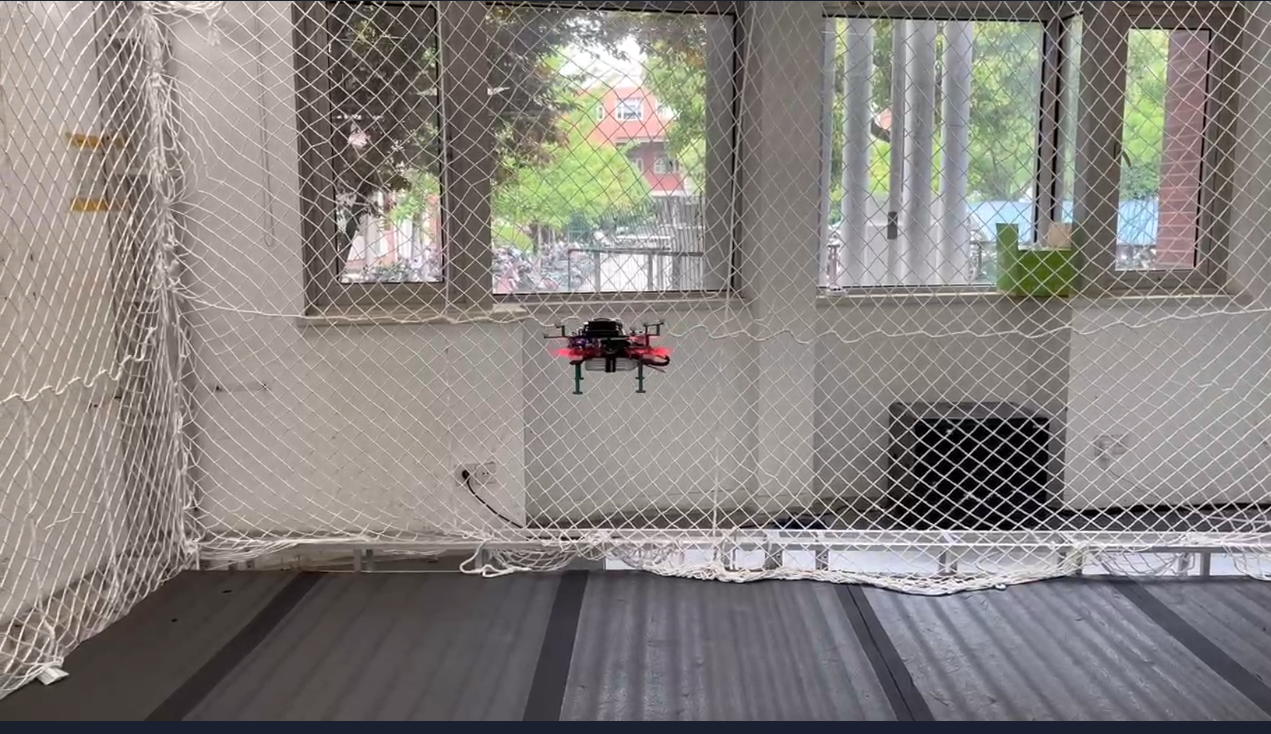
\includegraphics[width=0.95\linewidth]{室内飞行1.png}
  \end{subfigure} \hfill
  \begin{subfigure}[c]{0.33\textwidth}
    \centering
    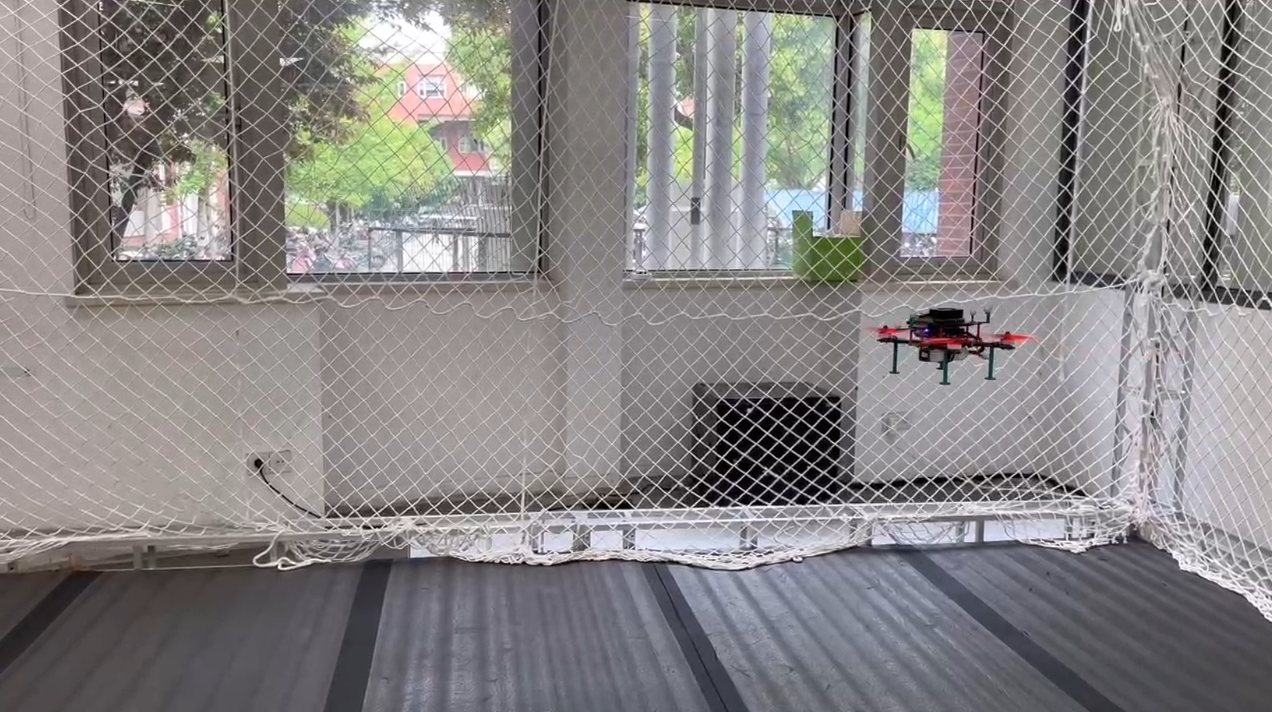
\includegraphics[width=0.95\linewidth]{室内飞行2.png}
  \end{subfigure}\hfill
    \begin{subfigure}[c]{0.33\textwidth}
      \centering
      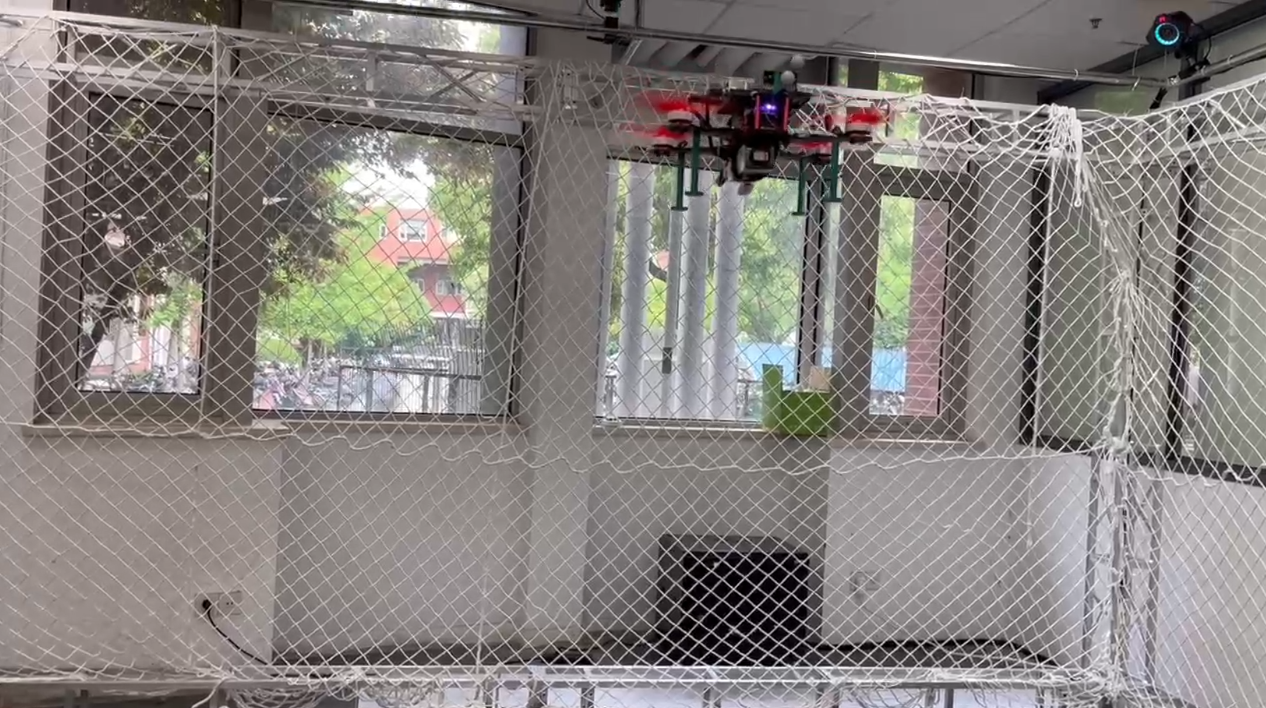
\includegraphics[width=0.95\linewidth]{室内飞行3.png}
  \end{subfigure}
  \caption{位置模式下四旋翼室内飞行画面}
  \label{室内飞行}
  \end{figure}
\newpage
  \section{四旋翼转动惯量测定}
  在仿真实验一章的硬件在环仿真节中得到的飞控固件就可以直接用于实机飞行,但在起飞前还需要做一些准备工作。
  HOFA算法需要知道无人机的转动惯量矩阵作为先验信息。经过仿真发现,HOFA算法可以容忍较大的转动惯量误差,但如果误差达到十倍的程度,还是会带来破坏性的影响。因此,需要对无人机进行较为精确的转动惯量测定。

  由于四旋翼大体是中心对称结构,因此只考虑转动惯量矩阵对角线上的元素,即中心主转动惯量。主转动惯量可以采用双线摆方法测量\cite{转动惯量}:用两条长度为 $L$ 的细线悬垂待测物体,两细线竖直,间隔距离为$d$,使待测转轴与两线竖直中心线重合,绕转轴轻轻拨动待测物体,使其有 $10 ^\circ$ 以下的转角,记录其摆动五十个周期的时间,重复三次。

  双线摆动能势能之和对时间求导为$0$,得到形如$kx+m\ddot x=0$的方程。易得,转动惯量与周期之间的关系为
  $$
  J_{ii}=\frac{mgd^2}{16 \pi^2 L} T^2
  $$
其中无人机质量$m$由电子天平测得为$0.8771kg$,上海地区重力加速度为$9.794 m/s^2$。用双线法分别测量无人机绕X轴,Y轴,Z轴的主转动惯量,如图\ref{双线法}所示。
  \begin{figure}[H]
    \centering
    \begin{subfigure}[c]{0.33\textwidth}
      \centering
      \includegraphics[width=0.95\linewidth, angle=270]{x.jpg}  % 确保角度为0
      \caption{X轴}
    \end{subfigure}\hfill
    \begin{subfigure}[c]{0.33\textwidth}
      \centering
      \includegraphics[width=0.95\linewidth, angle=270]{y.jpg}  % 确保角度为0
      \caption{Y轴}
    \end{subfigure}\hfill
    \begin{subfigure}[c]{0.33\textwidth}
      \centering
      \includegraphics[width=0.95\linewidth, angle=270]{z.jpg}  % 确保角度为0
      \caption{Z轴}
    \end{subfigure}
    \caption{双线法测量无人机主转动惯量}
    \label{双线法}
\end{figure}
用以上方法重复测量三次并计算,得到的原始数据和计算结果在表\ref{三次}中呈现。最终得到结论$J=\begin{bmatrix}
  0.0031 &0&0\\
  0&0.0032&0\\
  0&0& 0.0045
\end{bmatrix}kg \cdot m^2$,这与理论计算的估计差异不大。
  \begin{table}[H]
    \centering
    \caption{无人机转动惯量矩阵主值测量记录表}
    \label{三次}
    \begin{tabular}{cccccccc}
        \toprule
        组别&d/m  & L/m & 50T/s (1) & 50T/s (2) &50T/s (3) & T/s & $J_{ii} / kg \cdot m^2$\\
        \midrule
        $J_{xx}$ & 0.209 &0.67 & 46.46 & 46.36 & 46.40 &0.9281 &0.0031\\
        $J_{yy}$ & 0.170 &0.66 & 58.40 & 57.96 & 58.37 &1.1649 &0.0032\\
        $J_{zz}$ & 0.271 & 0.65& 42.50 & 42.75 & 42.75 &0.8533 &0.0045\\
        \bottomrule
    \end{tabular}
\end{table}

\section{开源飞控现实飞行信号分析}
由于时间的限制,我们尚未能解决HOFA实飞实验中遇到的一系列工程问题,仅仅完成了PX4原生固件的Offboard实飞。但通过分析其飞行日志记录的各种数据,也能得到对后续HOFA工程改进的有效意见。

\begin{figure}[!h]
  \centering
    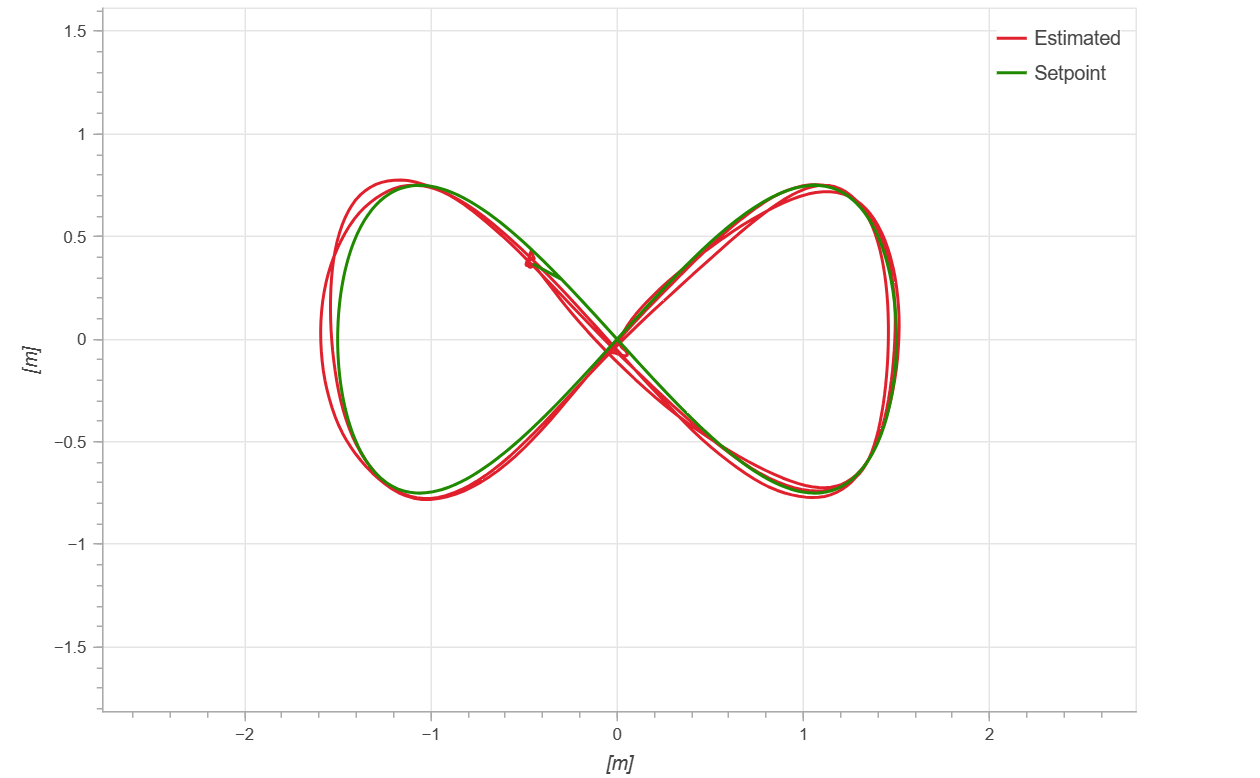
\includegraphics[width=0.5\textwidth]{real_px4_3d.png}
    \caption{PX4实飞轨迹曲线}
    \label{real_px4_3d}
  \end{figure}
  \begin{figure}[!h]
    \centering
      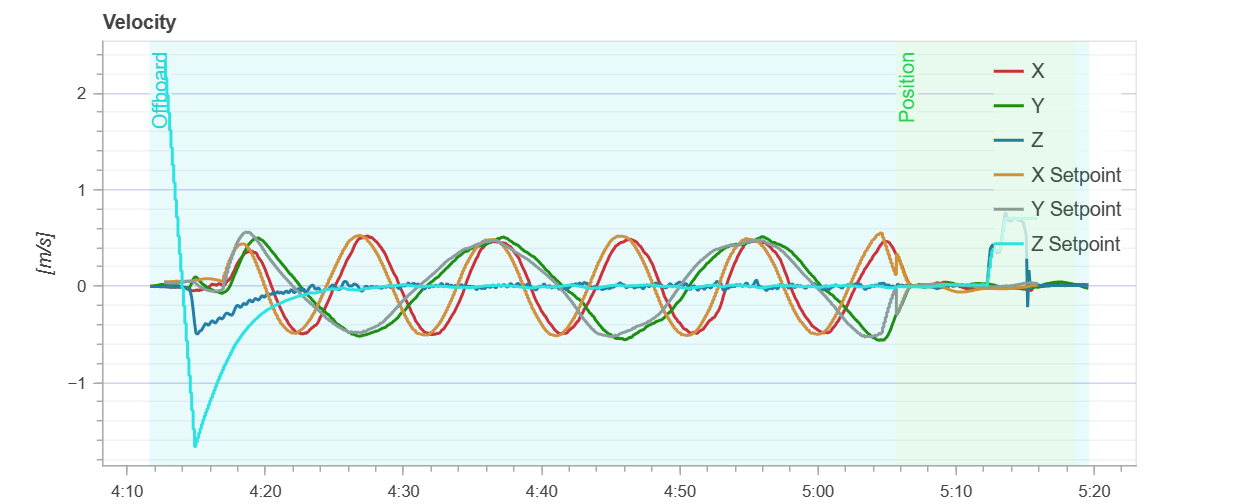
\includegraphics[width=0.6\linewidth]{real_px4_v.png}
      \caption{PX4实飞速度曲线}
      \label{real_px4_v}

\end{figure}



如图\ref{real_px4_3d}和图\ref{real_px4_v}所示,PX4对“8”字型轨迹有良好的跟踪效果,速度和期望速度都较为平稳。进一步地,我们从中分析HOFA在实飞中会遇到的问题以及原因,并尝试给出下一步的解决方案。由于HOFA与PX4的位置环相同,这也意味着在姿态环表现良好时,$x_d,v_d,x,v$都会是性质良好的平滑曲线,故而有理由推测解算出的期望姿态也是较为平滑的。在图\ref{real_px4_wdw}中也确实可以看到,此时产生的期望姿态是大体平稳的,波动的幅度可以接受。但对期望姿态做一次微分得到的期望角速度就已经有了不小的抖动,如果再做一次微分得到期望角加速度,信号中的噪声必然会更严重。加之两次微分在实际操作中是由前后两次的上级信号差分而来,得到的期望角加速度就会有叠加的延迟,加剧前馈补偿的失真。另外,角速度的估计存在剧烈的波动,无论这是因为传感器的采样噪声还是电机的振动使得IMU确实有高频的角速度变化,这种高频且幅值较大的波动都会对HOFA控制提出挑战。一方面是HOFA的前馈补偿中存在角速度和期望角速度的二次项,大的赋值会被二次项放大,另一方面,角速度的快速变动对控制频率和延迟也有很高的要求。


\begin{figure}[!h]
  \centering
  \begin{subfigure}[b]{0.49\textwidth}
      \centering
      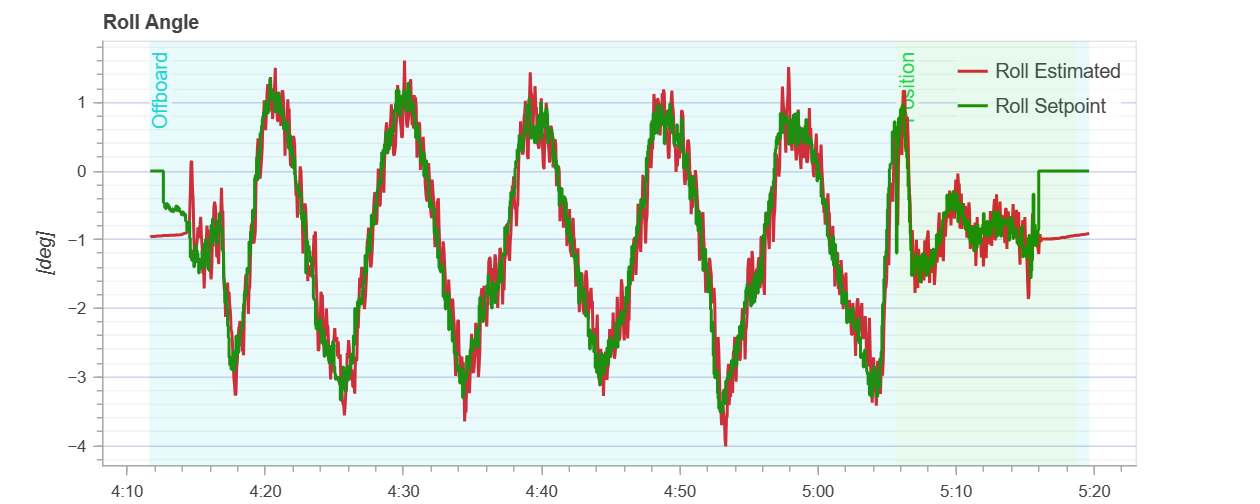
\includegraphics[width=\linewidth]{real_px4_w1.png}
      \caption{$\omega_1$}
  \end{subfigure}
  \hfill
  \begin{subfigure}[b]{0.49\textwidth}
      \centering
      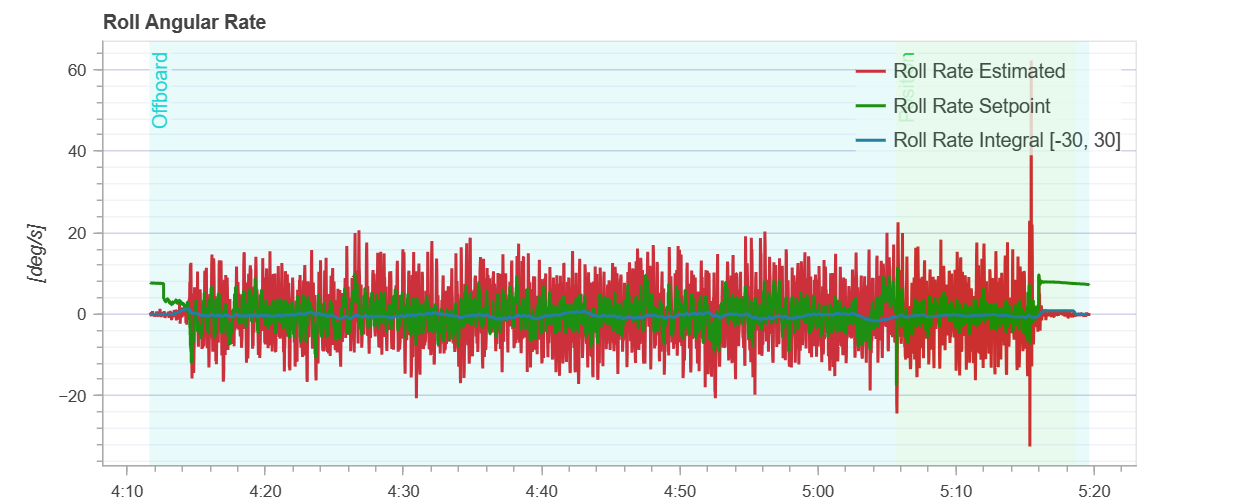
\includegraphics[width=\linewidth]{real_px4_dw1.png}
      \caption{$\dot \omega_1$}
  \end{subfigure}
  
  \begin{subfigure}[b]{0.49\textwidth}
      \centering
      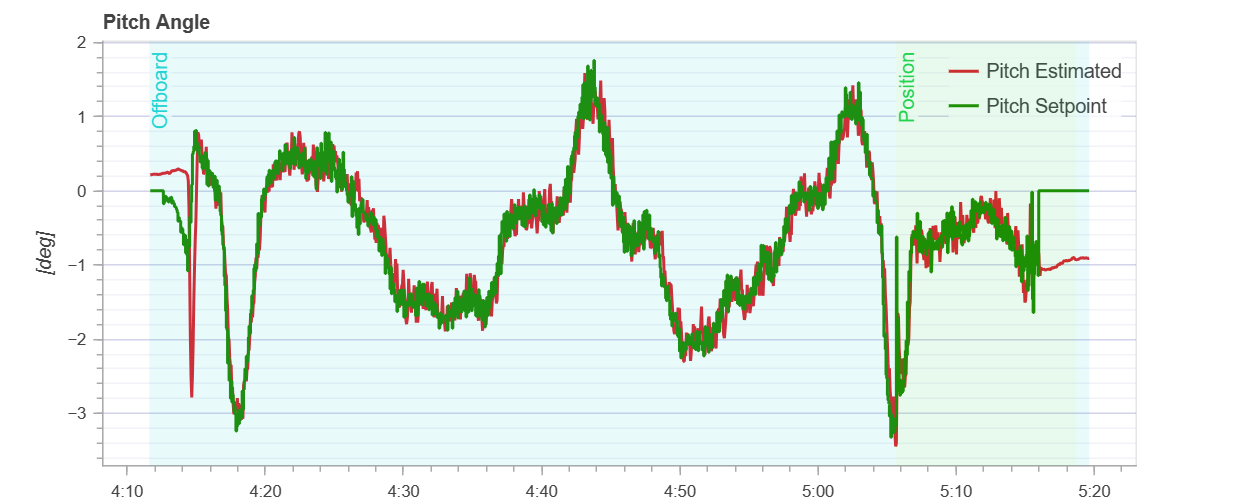
\includegraphics[width=\linewidth]{real_px4_w2.png}
      \caption{$\omega_2$}
  \end{subfigure}
  \hfill
  \begin{subfigure}[b]{0.49\textwidth}
      \centering
      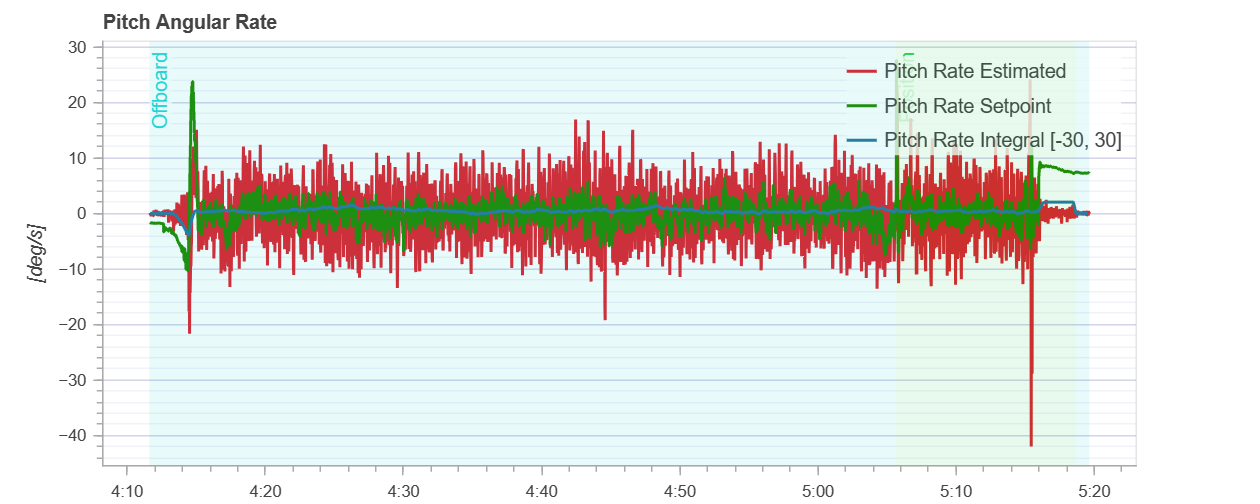
\includegraphics[width=\linewidth]{real_px4_dw2.png}
      \caption{$\dot \omega_2$}
  \end{subfigure}
  
  \begin{subfigure}[b]{0.49\textwidth}
      \centering
      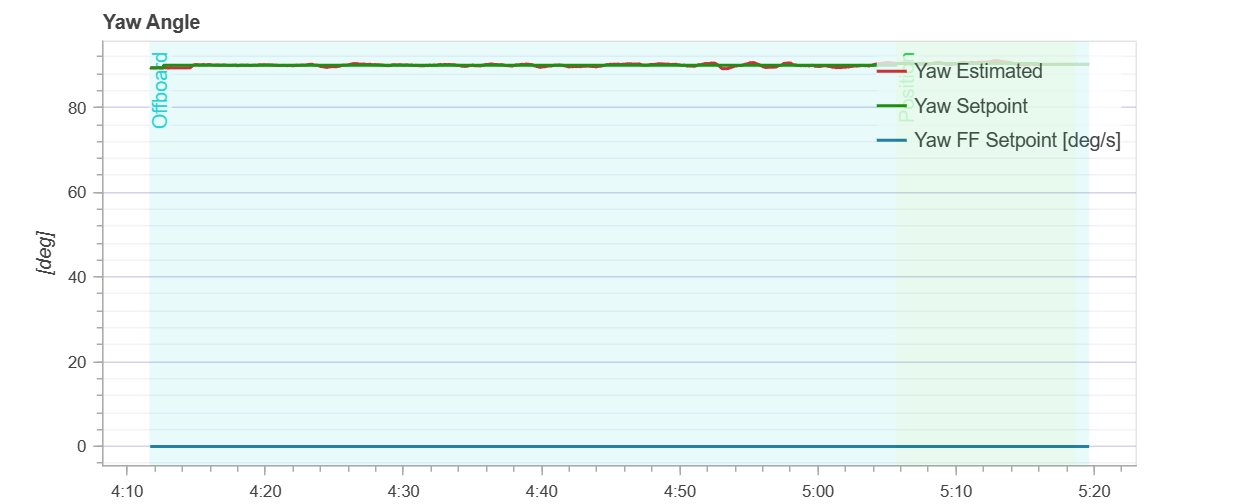
\includegraphics[width=\linewidth]{real_px4_w3.png}
      \caption{$\omega_3$}
  \end{subfigure}
  \hfill
  \begin{subfigure}[b]{0.49\textwidth}
      \centering
      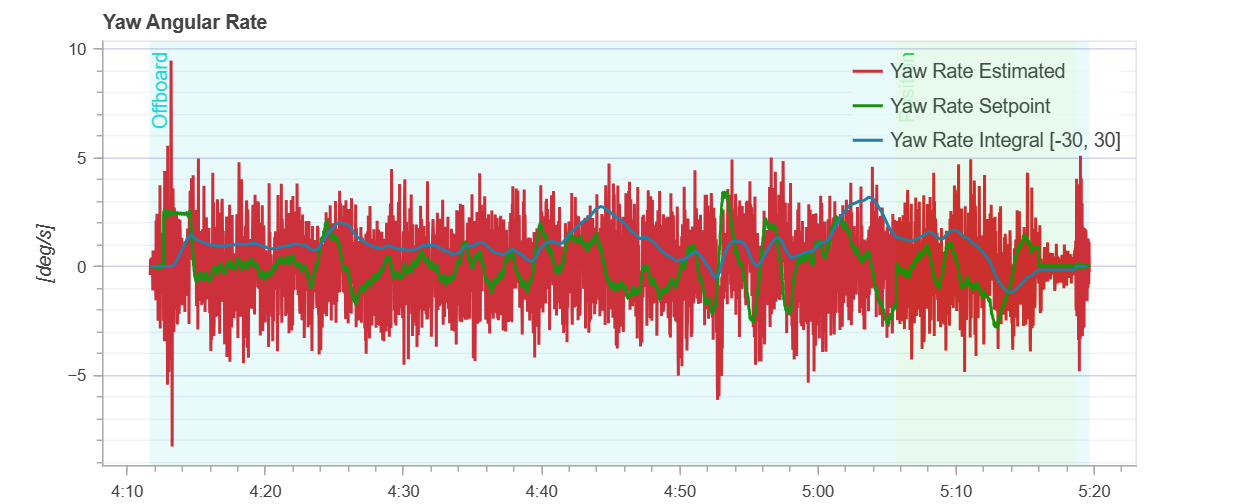
\includegraphics[width=\linewidth]{real_px4_dw3.png}
      \caption{$\dot \omega_3$}
  \end{subfigure}
  \caption{PX4实飞角度和角速度曲线}
  \label{real_px4_wdw}
\end{figure}

最后来看输出,如图\ref{real_px4_fM}和图\ref{real_px4_f1234},力矩一直有高频波动但幅值不超过$0.1N\cdot m$,这可以作为限幅的参考。电机的控制指令也一直没有超过$50\%$,因此在控制器足够好的情况下,这台无人机能够进行更为激进的飞行。
\begin{figure}[!h]
  \centering
  \begin{minipage}[b]{0.49\linewidth}
      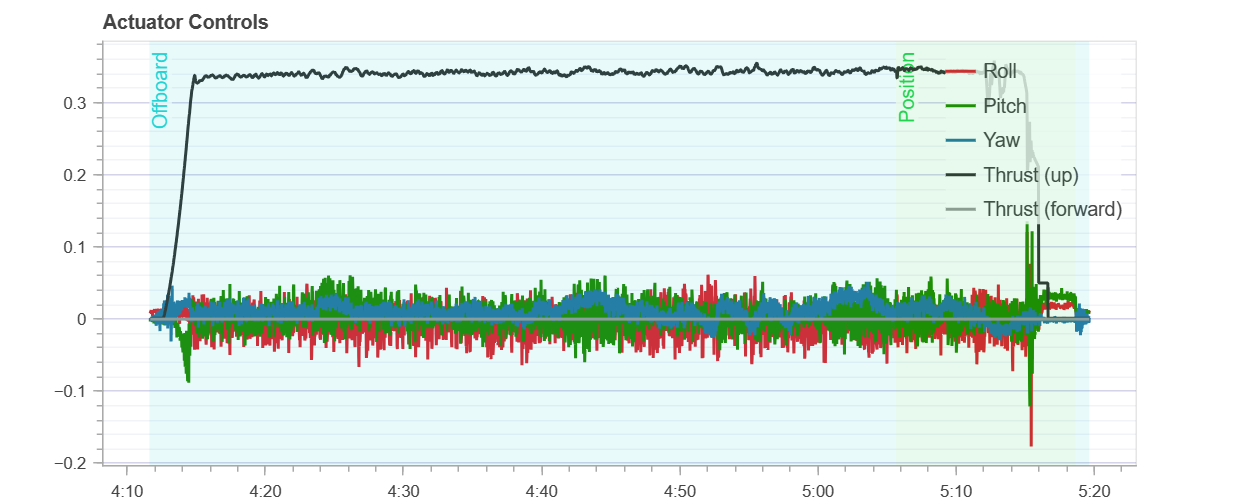
\includegraphics[width=\linewidth]{real_px4_fM.png}
      \caption{PX4实飞运动控制输出}
      \label{real_px4_fM}
  \end{minipage}
  \hfill % 在图片之间添加一些空间
  \begin{minipage}[b]{0.49\linewidth}
      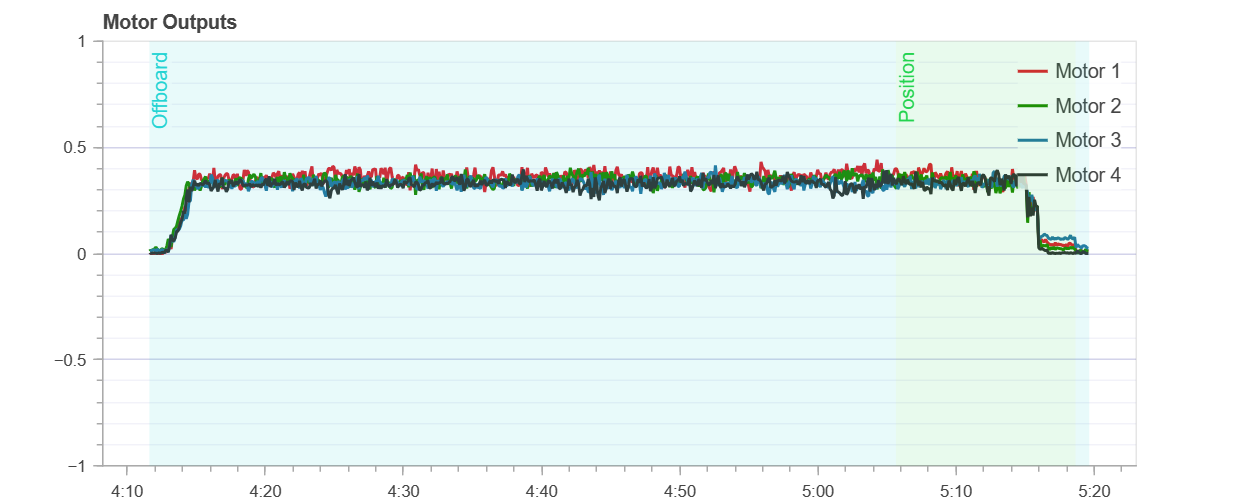
\includegraphics[width=\linewidth]{real_px4_f1234.png}
      \caption{PX4实飞电机指令}
      \label{real_px4_f1234}
  \end{minipage}
\end{figure}


PX4的官方文档中称其位置环的控制频率为50Hz,姿态控制频率为250Hz,角速度为1000Hz\cite{px4}。但因为其架构过于复杂,我始终未能找到其进程安排的代码,故而只能在飞行日志的数据中根据时间戳来看各环节的频率作为参考,记录在表\ref{频率}。这里的频率是飞控向外发布记录数据的频率,并不是内部实际的控制频率,并且这个频率并不严格,会有多至$10\%$的波动,这应该受硬件算力波动的影响。
\begin{table}[!h]
  \centering
  \caption{PX4实飞各信号发布频率}
  \label{频率}
  \begin{tabular}{cccccccccc}
      \toprule
      信号&$x$ & $x_d$ & $v$ &$v_d$ &$R$ &$R_d$& $\omega$ &$\omega_d$ &$M$\\
      \midrule
频率(Hz)&10& 10& 10& 10& 20&20& 50 & 50&50\\
      \bottomrule
  \end{tabular}
\end{table}


\section{本章小节}
本章描述了实机飞行平台的完整搭建过程,从室外飞行,到室内基于动捕的飞行,到用Offboard程序发布轨迹。虽然HOFA的实机飞行由于时间有限,还有工程问题需要解决,但也通过PX4原生固件的飞行数据,结合前文的仿真结果,给出了分析和改进方法。当前实机HOFA飞行效果不佳的可能原因有以下三点:
1)两阶微分求得的期望角加速度会放大噪声的延迟的不良影响;
2)高频大幅度波动的角速度会被前馈补偿中的二次项放大
3)对PX4固件的改写在线程管理上尚有优化余地,控制频率还能进一步提高。这些都是未来研究工作中需要着重解决的难点。

